\chapter{Giant Molecular Clouds}
\label{ch:gmcs}

\marginnote{
\textbf{Suggested background reading:}
\begin{itemize}
\item \href{http://adsabs.harvard.edu/abs/2014prpl.conf....3D}{Dobbs, C.~L., et al. 2014, in ``Protostars and Planets VI", ed.~H.~Beuther et al., pp.~3-26} \nocite{dobbs14a}
\end{itemize}
\textbf{Suggested literature:}
\begin{itemize}
\item \href{http://adsabs.harvard.edu/abs/2014ApJ...784....3C}{Colombo, D., et al. 2014, ApJ, 784, 3} \nocite{colombo14a}
\end{itemize}
}

We now begin our top-down study of star formation, from large to small scales. This chapter focuses on observations of the bulk properties of giant molecular clouds (GMCs), primarily in the Milky Way and in nearby galaxies where we can resolve individual GMCs. The advantage of looking at the Milky Way is of course higher resolution. The advantage of looking at other galaxies is that, unlike in the Milky Way, we can get an unbiased view of all the GMCs, with much smaller distance uncertainties and many fewer confusion problems. This allows us to make statistical inferences that are often impossible to check with confidence locally. This study will be a preparation for the next two chapters, which discuss the correlation of molecular clouds with star formation and the problem of the star formation rate.

\section{Molecular Cloud Masses}

\subsection{Mass Measurement}

The most basic quantity we can measure for a molecular cloud is its mass. However, this also turns out to be one of the trickiest quantities to measure. The most commonly used method for inferring masses is based on molecular line emission, because lines are bright and easy to see even in external galaxies. The three most commonly-used species on the galactic scale are $^{12}$CO, $^{13}$CO, and, more recently, HCN.

\paragraph{Optically Thin Lines}

Conceptually, $^{13}$CO is the simplest, because its lines are generally optically thin. For emitting molecules in LTE at temperature $T$, it is easy to show from the radiative transfer equation that the intensity emitted by a cloud of optical depth $\tau_{\nu}$ at frequency $\nu$ is simply
\begin{equation}
I_{\nu} = \left(1-e^{-\tau_{\nu}}\right) B_{\nu}(T),
\end{equation}
where $B_{\nu}(T)$ is the Planck function evaluated at frequency $\nu$ and temperature $T$.

Although we will not derive this equation here\footnote{See any standard radiative transfer reference, for example \citet{rybicki86a} or \citet{shu91a}.}, it behaves exactly as one would expect intuitively. In the limit of a very optically thick cloud, $\tau_{\nu}\gg 1$, the exponential factor becomes zero, and the intensity simply approaches the Planck function, which is the intensity emitted by a black body. In the limit of a very optically thin cloud, $\tau_{\nu}\ll 1$, the exponential factor just becomes $1-\tau_{\nu}$, so the intensity approaches that of a black body multiplied by the (small) optical depth. Thus the intensity is simply proportional to the optical depth, which is proportional to the number of atoms along the line of sight.

These equations allow the following simple method of deducing the column density from an observation of the $^{13}$CO and $^{12}$CO $J=1\rightarrow 0$ lines (or any similar pair of $J$ lines) from a molecular cloud. If we assume that the $^{12}$CO line is optically thick, as is almost always the case, then we can approximate $1-e^{-\tau_{\nu}}\approx 1$ at line center, so $I_{\nu} \approx B_{\nu}(T)$. If we measure $I_{\nu}$, we can therefore immediately deduce the temperature $T$. We then assume that the $^{13}$CO molecules are at the same temperature, so that $B_{\nu}(T)$ is the same for $^{12}$CO and $^{13}$CO except for the slight shift in frequency. Then if we measure $I_\nu$ for the center of the $^{13}$CO line, we can solve the equation
\begin{equation}
I_{\nu} = \left(1-e^{-\tau_{\nu}}\right) B_{\nu}(T),
\end{equation}
for $\tau_{\nu}$, the optical depth of the $^{13}$CO line. If $N_{\rm ^{13}CO}$ is the column density of $^{13}$CO atoms, then for gas in LTE the column densities of atoms in the level 0 and 1 states are
\begin{eqnarray*}
N_0 & = & \frac{N_{^{13}CO}}{Z} \\
N_1 & = & e^{-T/T_1}\frac{N_{^{13}CO}}{Z}
\end{eqnarray*}
where $Z$ is the partition function, which is a known function of $T$, and $T_1=5.3$ K is the temperature corresponding to the first excited state.

The opacity to line absorption at frequency $\nu$ is
\begin{equation}
\kappa_{\nu} = \frac{h\nu}{4\pi} (n_0 B_{01} - n_1 B_{10}) \phi(\nu),
\end{equation}
where $B_{01}$ and $B_{10}$ are the Einstein coefficients for spontaneous absorption and stimulated emission, defined by 
\begin{eqnarray}
B_{10} & = & \frac{c^2}{2 h \nu^3} A_{10} \\
B_{01} & = & \frac{g_1}{g_0} B_{10}.
\end{eqnarray}
The quantity $\phi(\nu)$ is the line shape function (see Chapter \ref{ch:obscold}). The corresponding optical depth at line center is
\begin{equation}
\tau_{\nu} = \frac{h\nu}{4\pi} (N_0 B_{01} - N_1 B_{10}) \phi(\nu).
\end{equation}
Since we know $\tau_{\nu}$ from the line intensity, we can measure $\phi(\nu)$ just by measuring the shape of the line, and $N_0$ and $N_1$ depend only on $N_{\rm ^{13}CO}$ and the (known) temperature, we can solve for $N_{\rm ^{13}CO}$.  In practice we generally do this in a slightly more sophisticated way, by fitting the optical depth and line shape as a function of frequency simultaneously, but the idea is the same. We can then convert to an H$_2$ column density by assuming a ratio of $^{12}$CO to H$_2$, and of $^{13}$CO to $^{12}$CO.

This method also has some significant drawbacks that are worth mentioning. The need to assume ratios of $^{13}$CO to $^{12}$CO and $^{12}$CO to H$_2$ are obvious ones. The former is particularly tricky, because there is strong observational evidence that the $^{13}$C to $^{12}$C ratio varies with galactocentric radius. We also need to assume that the $^{12}$CO and $^{13}$CO molecules are at the same temperature, which may not be true because the $^{12}$CO emission comes mostly from the cloud surface and the $^{13}$CO comes from the entire cloud. Since the cloud surface is usually warmer than its deep interior, this will tend to make us overestimate the excitation temperature of the $^{13}$CO molecules, and thus underestimate the true column density. This problem can be even worse because the lower abundance of $^{13}$CO means that it cannot self-shield against dissociation by interstellar UV light as effectively at $^{12}$CO. As a result, it may simply not be present in the outer parts of clouds at all, leading us to miss their mass and underestimate the true column density.

Another serious worry is the assumption that the $^{13}$CO molecules are in LTE. As shown in Problem Set 1, the $^{12}$CO $J=1$ state has a critical density of a few thousand cm$^{-3}$, which is somewhat above the mean density in a GMC even when we take into account the effects of turbulence driving mass to high density. The critical density for the $^{13}$CO $J=1$ state is similar. For the $^{12}$CO $J=1$ state, the effective critical density is lowered by optical depth effects, which thermalize the low-lying states. Since $^{13}$CO is optically thin, however, there is no corresponding thermalization for it, so in reality the excitation of the gas tends to be sub-LTE. The result is that the emission is less than we would expect based on an LTE assumption, and so we tend to underestimate the true $^{13}$CO column density, and thus the mass, using this method.

A final point to mention about this method is that, since the $^{13}$CO line is optically thin, it is simply not as bright as an optically thick line would be. Consequently, this method is generally only used within the Galaxy, not for external galaxies.

\paragraph{Optically Thick Lines}

Optically thick lines are nice and bright, so we can see them in distant galaxies. The challenge for an optically thick line is how to infer a mass, given that we are really only seeing the surface of a cloud. Our standard approach here is to define an "X factor": a scaling between the observed frequency-integrated intensity along a given line of sight and the column density of gas along that line of sight. For example, if we see a frequency-integrated CO $J=1\rightarrow 0$ intensity $I_{\rm CO}$ along a given line of sight, we define $X_{\rm CO}=N/I_{\rm CO}$, where $N$ is the true column density (in H$_2$ molecules per cm$^2$) of the cloud. Note that radio astronomers work in horrible units, so the X factor is defined in terms of a velocity-integrated brightness temperature, rather than a frequency-integrated intensity -- specifically, the usual units for $X_{\rm CO}$ are $\mbox{cm}^{-2} / (\mbox{K km s}^{-1})$. The brightness temperature corresponding to a given intensity at frequency $\nu$ is just defined as the temperature of a blackbody that produces that intensity at that frequency. Integrating over velocity just means that we integrate over frequency, but that we measure the frequency in terms of the Doppler shift in velocity it corresponds to.

The immediate question that occurs to us after defining the X factor is: why should such a scaling exist at all? Given that the cloud is optically thick, why should there be a relation between column density and intensity at all? On the face of it, this is a bit like claiming that the brightness of the thermal emission from a wall in a building is somehow related to the thickness of that wall. The reason this works is that a spectral line, even an optically thick one, contains much more information than continuum emission. Consider optically thick line emission from a cloud of mass $M$ and radius $R$ at temperature $T$. The mean column density is $N= M/(\mu m_{\rm H} \pi R^2)$, where $\mu=2.3$ is the mass per H$_2$ molecule in units of $m_{\rm H}$. The total integrated intensity we expect to see from the line is
\begin{equation}
\int I_{\nu}\, d\nu = \int (1 - e^{-\tau_{\nu}}) B_{\nu}(T)\,d\nu.
\end{equation}

Suppose this cloud is in virial balance between kinetic energy and gravity, i.e., $\mathcal{T}=\mathcal{W}/2$ so that $\ddot{I}=0$, neglecting magnetic and surface terms. The gravitational-self energy is $\mathcal{W}=a GM^2/R$, where $a$ is a constant of order unity that depends on the cloud's geometry and internal mass distribution. For a uniform sphere $a=3/5$. The kinetic energy is $\mathcal{T}=(3/2)M\sigma_{\rm 1D}^2$, where $\sigma_{\rm 1D}$ is the one dimensional velocity dispersion, including both thermal and non-thermal components.

We define the observed virial ratio as
\begin{equation}
\label{eq:alpha_vir_obs}
\avir =  \frac{5\sigma_{\rm 1D}^2 R}{GM}.
\end{equation}
For a uniform sphere, which has $a=3/5$, this definition reduces to $\avir=2\mathcal{T}/\mathcal{W}$, which is the virial ratio we defined previously based on the virial theorem (equation \ref{eq:alpha_vir_th}). Thus $\avir=1$ corresponds to the ratio of kinetic to gravitational energy in a uniform sphere of gas in virial equilibrium between internal motions and gravity. In general we expect that $\avir\approx 1$ in any object supported primarily by internal turbulent motion, even if its mass distribution is not uniform.

Re-arranging this definition, we have
\begin{equation}
\sigma_{\rm 1D} = \sqrt{\left(\frac{\avir}{5}\right)\frac{GM}{R}}.
\end{equation}
To see why this is relevant for the line emission, consider the total frequency-integrated intensity that the cloud will emit in the line of interest. We have as before
\begin{equation}
I_{\nu} = \left(1-e^{-\tau_{\nu}}\right) B_{\nu}(T),
\end{equation}
so integrating over frequency we get
\begin{equation}
\int I_{\nu}\,d\nu = \int \left(1-e^{-\tau_{\nu}}\right) B_{\nu}(T)\,d\nu.
\end{equation}
The optical depth at line center is $\tau_{\nu_0}\gg 1$, and for a Gaussian line profile the optical depth at frequency $\nu$ is
\begin{equation}
\tau_{\nu} =\tau_{\nu_0} \exp\left[-\frac{(\nu-\nu_0)^2}{2 (\nu_0 \sigma_{\rm 1D}/c)^2}\right],
\end{equation}
where $\nu_0$ is the frequency of line center. Since the integrated intensity depends on the integral of $\tau_{\nu}$ over frequency, and the frequency-dependence of $\tau_{\nu}$ is determined by $\sigma_{\rm 1D}$, we therefore expect that the integrated intensity will depend on $\sigma_{\rm 1D}$.  

To get a sense of how this dependence will work, let us adopt a very simplified yet schematically correct form for $\tau_{\nu}$. We will take the opacity to be a step function, which is infinite near line center and drops sharply to 0 far from line center. The frequency at which this transition happens will be set by the condition $\tau_{\nu}=1$, which gives
\begin{equation}
\Delta \nu = |\nu-\nu_0| = \nu_0 \sqrt{2\ln \tau_{\nu_0}} \frac{\sigma_{\rm 1D}}{c}.
\end{equation}
The corresponding range in Doppler shift is
\begin{equation}
\Delta v = \sqrt{2\ln \tau_{\nu_0}} \sigma_{\rm 1D}.
\end{equation}
For this step-function form of $\tau_{\nu}$, the emitted brightness temperature is trivial to compute. At velocity $v$, the brightness temperature is
\begin{equation}
T_{B,v} = \left\{
\begin{array}{ll}
T, \qquad & |v-v_0| < \Delta v \\
0, &  |v-v_0| > \Delta v
\end{array}
\right.,
\end{equation}
where $v_0$ is the cloud's mean velocity.

If we integrate this over all velocities of emitting molecules, we get
\begin{equation}
I_{\rm CO} = \int T_{B,\nu}\, dv = 2 T_B \Delta v = \sqrt{8\ln\tau_{\nu_0}} \sigma_{\rm 1D} T.
\end{equation}
Thus, the velocity-integrated brightness temperature is simply proportional to $\sigma_{\rm 1D}$. The dependence on the line-center optical depth is generally negligible, since that quantity enters only as the square root of the log. We therefore have
\begin{eqnarray*}
X\mbox{ [cm}^{-2}\mbox{ (K km s}^{-1}\mbox{)}^{-1}\mbox{]} & = & \frac{M/(\mu \pi R^2)}{I_{\rm CO}} \\
& = & 10^5 \frac{(8\ln\tau_{\nu_0})^{-1/2}}{T\mu\pi} \frac{M}{\sigma_{\rm 1D} R^2} \\
& = & 10^5 \frac{(\mu m_{\rm H} \ln\tau_{\nu_0})^{-1/2}}{T} \sqrt{\frac{5n}{6\pi \avir G}},
\end{eqnarray*}
where $n= 3M/(4\pi \mu m_{\rm H} R^3)$ is the number density of the cloud, and the factor of $10^5$ comes from the fact that we are measuring $I_{\rm CO}$ in km s$^{-1}$ rather than cm s$^{-1}$. To the extent that all molecular clouds have comparable volume densities on large scales and are virialized, this suggests that there should be a roughly constant CO X factor. If we plug in $T=10$ K, $n=100$ cm$^{-3}$, $\avir=1$, and $\tau_{\nu_0}=100$, this gives $X_{\rm CO}=5\times 10^{19}$ cm$^{-2}$ (K km s$^{-1}$)$^{-1}$.

This argument is a simplified version of a more general technique of converting between molecular line luminosity and mass called the large velocity gradient approximation, introduced by \citet{goldreich74a}. The basic idea of all these techniques is the same: for an optically thick line, the total luminosity that escapes will be determined not directly by the amount of gas, but instead by the range in velocity or frequency that the cloud occupies, multiplied by the gas temperature.

Of course this calculation has a few problems -- we have to assume a volume density, and there are various fudge factors like $a$ floating around. Moreover, we had to assume virial balance between gravity and internal motions. This implicitly assumes that both surface pressure and magnetic fields are negligible, which they may not be. Making this assumption would necessarily make it impossible to independently check whether molecular clouds are in fact in virial balance between gravity and turbulent motions.

In practice, the way we get around these problems is by determining X factors by empirical calibration. We generally do this by attempting to measure the total gas column density by some tracer that measures all the gas along the line of sight, and then subtracting off the observed atomic gas column -- the rest is assumed to be molecular.

One way of doing this is measuring $\gamma$ rays emitted by cosmic rays interacting with the ISM. The $\gamma$ ray emissivity is simply proportional to the number density of hydrogen atoms independent of whether they are in atoms or molecules (since the cosmic ray energy is very large compared to any molecular energy scales). Once produced, the $\gamma$ rays travel to Earth without significant attenuation, so the $\gamma$ ray intensity along a line of sight is simply proportional to the total hydrogen column. Using this method, \citet{strong96a} obtained $X \approx 2\times 10^{20}$ cm$^{-2}$ (K km s$^{-1}$)$^{-1}$, and more recent work from Fermi \citep{abdo10b} gives about the same value.

Another way is to measure the infrared emission from dust grains along the line of sight, which gives the total dust column. This is then converted to a mass column using a dust to gas ratio. Based on this technique, \citet{dame01a} obtained $X\approx 2 \times 10^{20}$ cm$^{-2}$ (K km s$^{-1}$)$^{-1}$; more recently, \citet{draine07a} got about twice this, $X\approx 4 \times 10^{20}$ cm$^{-2}$ (K km s$^{-1}$)$^{-1}$. However, all of these techniques give numbers that agree to within a factor of two in the Milky Way, so we can be fairly confident that the X factor works to that level. It is important to emphasize, however, that this is only under Milky Way conditions. We will see shortly that there is good evidence that it does not work under very different conditions.

Note that we can turn the argument around. These other calibration methods, which make no assumptions about virialization, give conversions that are in quite good agreement with what we get by assuming virialization between gravity and turbulence. This suggests that molecular clouds cannot be too far from virial balance between gravity and turbulence. Neither magnetic fields nor surface pressure can be completely dominant in setting their structures, nor can clouds have large values of $\ddot{I}$.

It is also worth mentioning some caveats with this method. The most serious one is that it assumes that CO will be found wherever H$_2$ is, so that the mass traced by CO will match the mass traced by H$_2$. This seems to be a pretty good assumption in the Milky Way, but it may begin to break down in lower metallicity galaxies due to the differences in how H$_2$ and CO are shielded against dissociation by the interstellar UV field.

\subsection{Mass Distribution}

Armed with these techniques for measuring molecular cloud masses, what do we actually see? The answer is that in both the Milky Way and in a collection of nearby galaxies, the molecular cloud mass distribution in the cloud seems to be well-fit by a truncated powerlaw,
\begin{equation}
\frac{d\mathcal{N}}{d M} =
\left\{
\begin{array}{ll}
\mathcal{N}_u \left(\frac{M_u}{M}\right)^{\gamma}, \qquad & M \leq M_u \\
0, & M > M_u
\end{array}
\right..
\end{equation}
Here $M_u$ represents an upper mass limit for GMCs -- there are no clouds in a galaxy larger than that mass. The number of clouds with masses near the upper mass limit is $N_u$. Below $M_u$, the mass distribution follows a powerlaw of slope $\gamma$. Note that, since we have given this as the number per unit log mass rather than the number per unit mass, we can think of this index as telling us the total mass of clouds per decade in mass.

\begin{marginfigure}
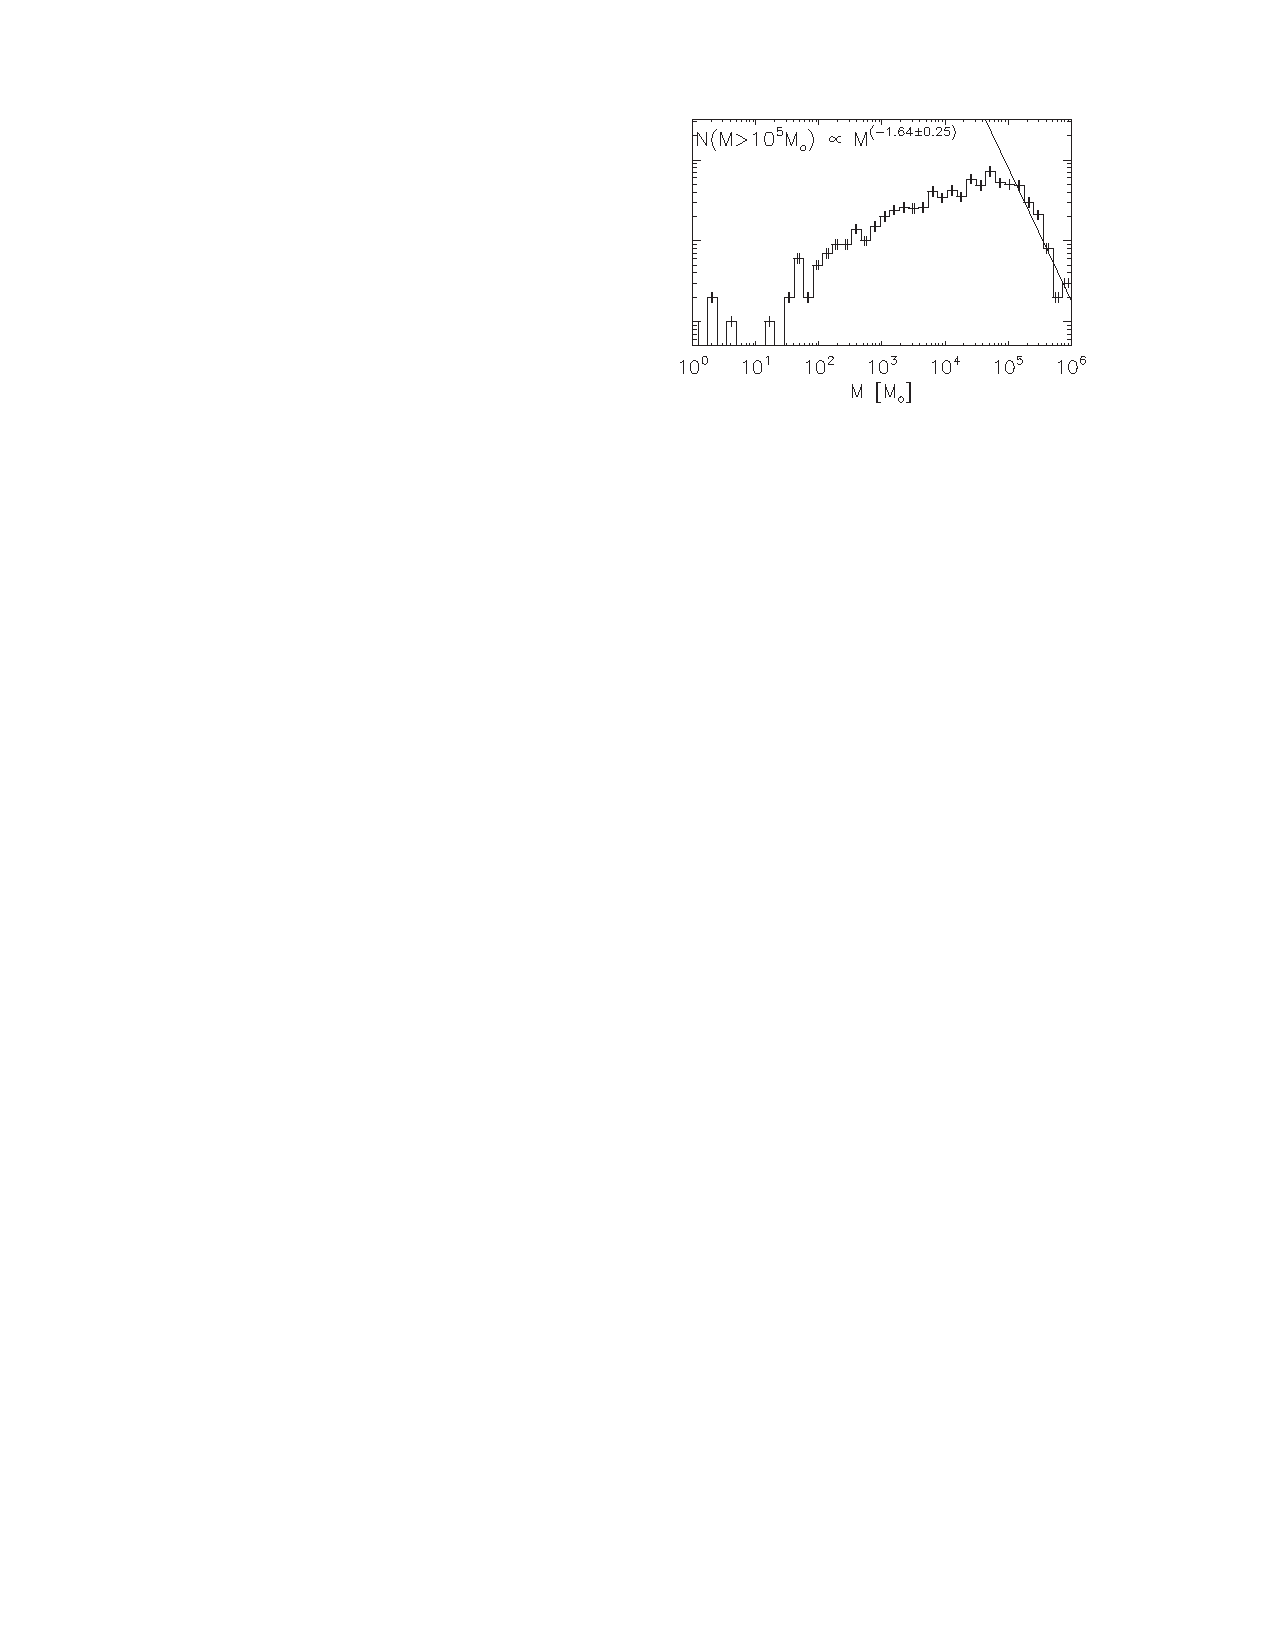
\includegraphics[width=\linewidth]{gmcmass_roman-duval}
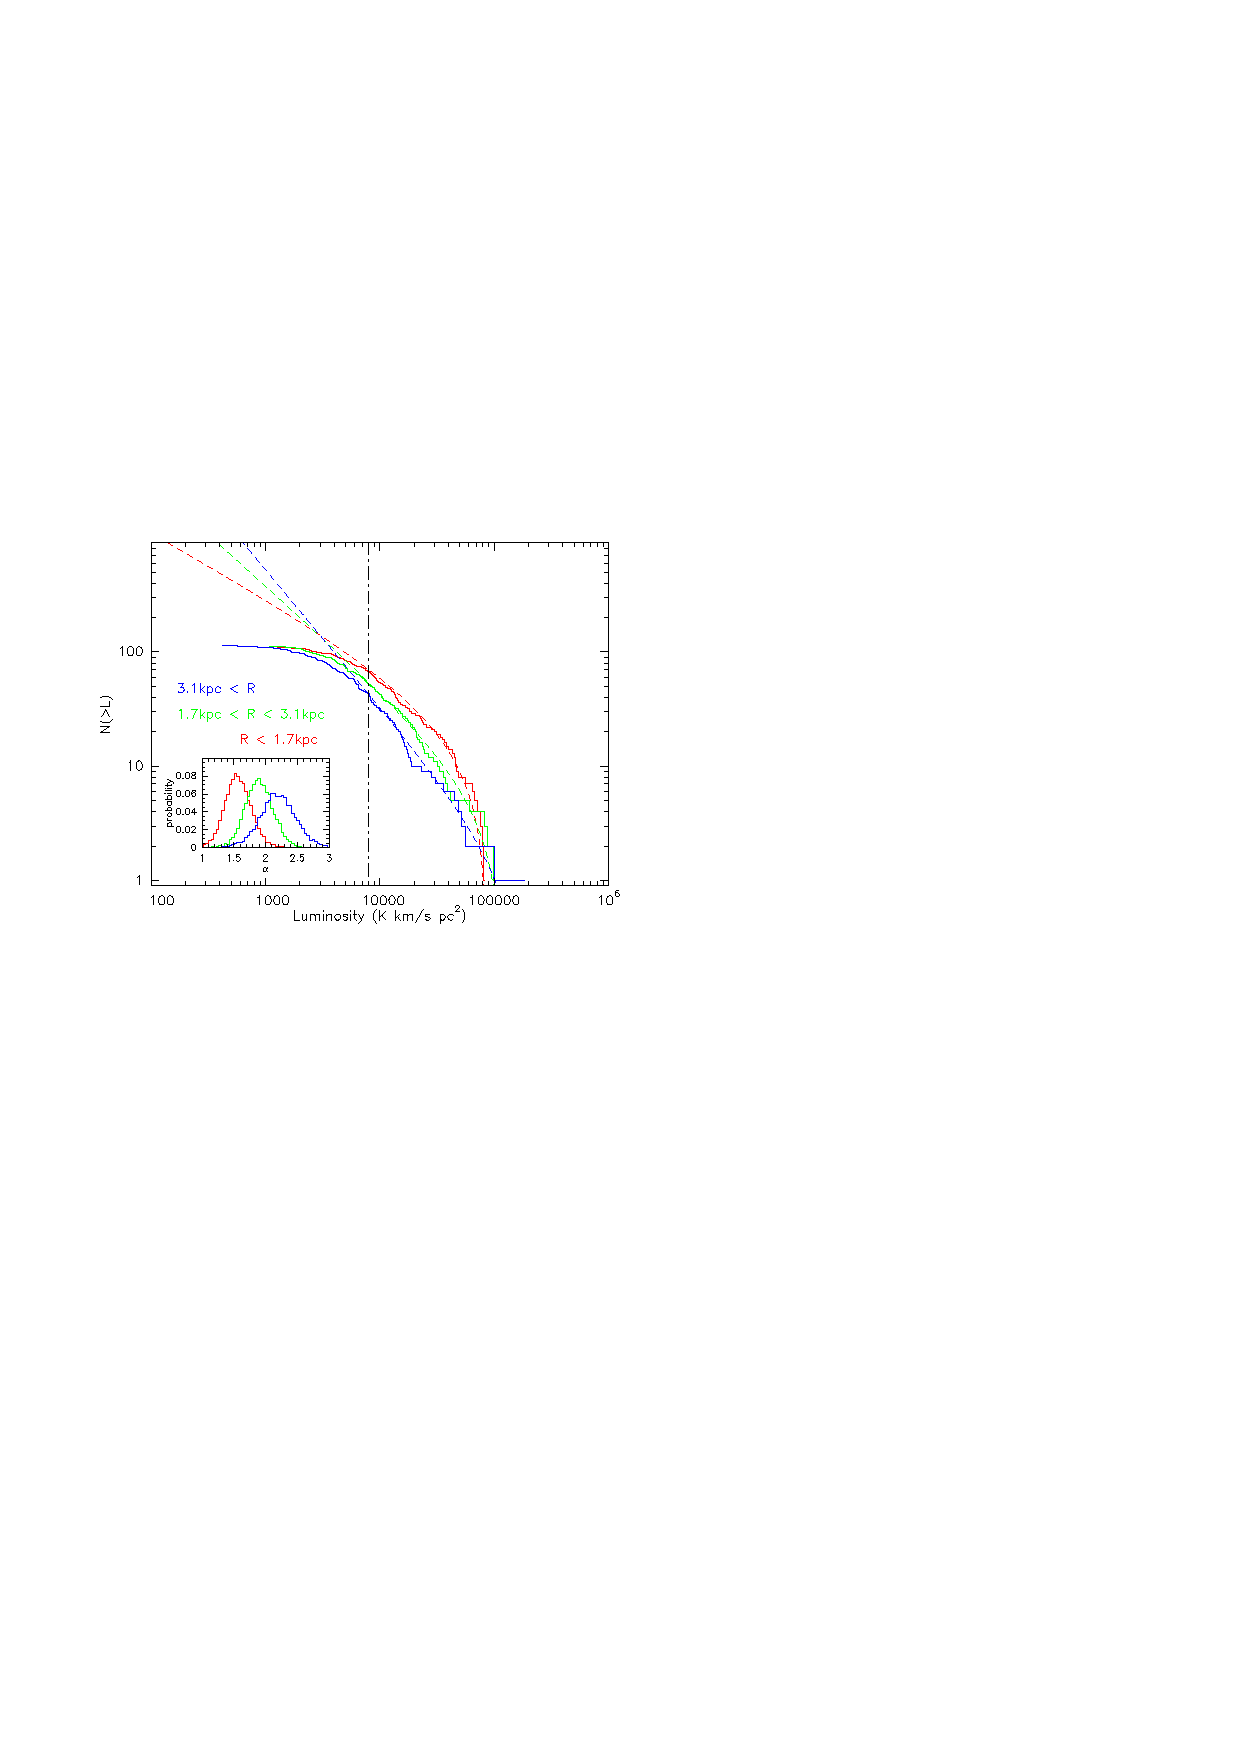
\includegraphics[width=\linewidth]{gmcmass_gratier}
\caption[GMC mass spectra]{
\label{fig:gmcmass}
Two measurements of the GMC mass spectrum. The top panel shows the mass spectrum for the inner Milky Way determined from $^{13}$CO measurements by \citet{roman-duval10a}; the sample is complete at masses above $\sim 10^5$ $M_\odot$. The bottom panel shows the mass spectrum in M33, as determined by \citet{gratier12a} using $^{12}$CO. Note that these are cumulative distributions in luminosity, whereas the top panel shows a differential distribution in mass. The three colors show three different galactocentric regions: the inner galaxy (red), the mid-disk (green), and the outer galaxy (blue).
}
\end{marginfigure}

So what are $N_u$, $M_u$, and $\gamma$? It depends on where we look, as illustrated in Figure \ref{fig:gmcmass}. In the inner, H$_2$-rich parts of galaxies, the slope is typically $\gamma \sim -2$ to $-1.5$. In the outer, molecule-poor regions of galaxies, and in dwarf galaxies, it is $-2$ to $-2.5$. These measurements imply that, since the bulk of the molecular mass is found in regions with $\gamma > -2$, most of the molecular mass is in large clouds rather than small ones. This is just because the mass in some mass range is proportional to $\int (d\mathcal{N}/dM) M \, dM \propto M^{2+\gamma}$. A value of $\gamma=-2$ therefore represents a critical line separating distributions that are dominated by large and small masses.

\section{Scaling Relations}

Once we have measured molecular cloud masses, the next thing to investigate is their other large-scale properties, and how they scale with mass. Observations of GMCs in the Milky Way and in nearby galaxies yield three basic results, which are known as Larson's Laws, since they were first pointed out by \citet{larson81a}. The physical significance of these observational correlations is still debated today.

The first is the molecular clouds have characteristic surface densities of $\sim 100$ $M_\odot$ pc$^{-2}$ (Figure \ref{fig:gmcsigma}). This appears to be true in the Milky Way and in all nearby galaxies where we can resolve individual clouds. There may be some residual weak dependence on the galactic environment -- $\sim 50$ $M_\odot$ pc$^{-2}$ in low surface density, low metallicity galaxies like the Large Magellanic Cloud (LMC), up $\sim 200$ $M_\odot$ pc$^{-2}$ in molecule- and metal-rich galaxies like M51, but generally around that value.

Note that the universal column density combined with the GMC mass spectrum implies are characteristic volume density for GMCs
\begin{equation}
n = \frac{3M}{4\pi R^3\mu m_{\rm H}} = \left(\frac{3\pi^{1/2}}{4\mu m_{\rm H}}\right) \sqrt{\frac{\Sigma^3}{M}} = 23 \Sigma_2^{3/2} M_6^{-1/2}\mbox{ cm}^{-2},
\end{equation}
where $\Sigma_2 = \Sigma/(100\,\msun\mbox{ pc}^{-2})$ and $M_6=M/10^6$ $\msun$. This is the number density of H$_2$ molecules, using a mean mass per molecule $\mu=2.3$. There is an important possible caveat to this, however, which is sensitivity bias: GMCs with surface densities much lower than this value may be hard to detect in CO surveys. However, there is no reason that higher surface density regions should not be detectable, so it seems fairly likely that this is a physical and not just observational result (though that point is disputed).

The second of Larson's Laws is that GMCs obey a linewidth-size relation. The velocity dispersion of a given cloud depends on its radius. \citet{solomon87a} find $\sigma = (0.72\pm 0.07)R_{\rm pc}^{0.5\pm 0.05}$ km s$^{-1}$ in the Milky Way, where $R_{\rm pc}$ is the cloud radius in units of pc. For a sample of a number of external galaxies, \citet{bolatto08a} find $\sigma = 0.44^{+0.18}_{-0.13} R_{\rm pc}^{0.60\pm 0.10}$ km s$^{-1}$. Within individual molecular clouds in the Milky Way, \citet{heyer04a} find $\sigma=0.9 L_{\rm pc}^{0.56\pm 0.02}$ km s$^{-1}$ (Figure \ref{fig:gmclws}).

\begin{marginfigure}
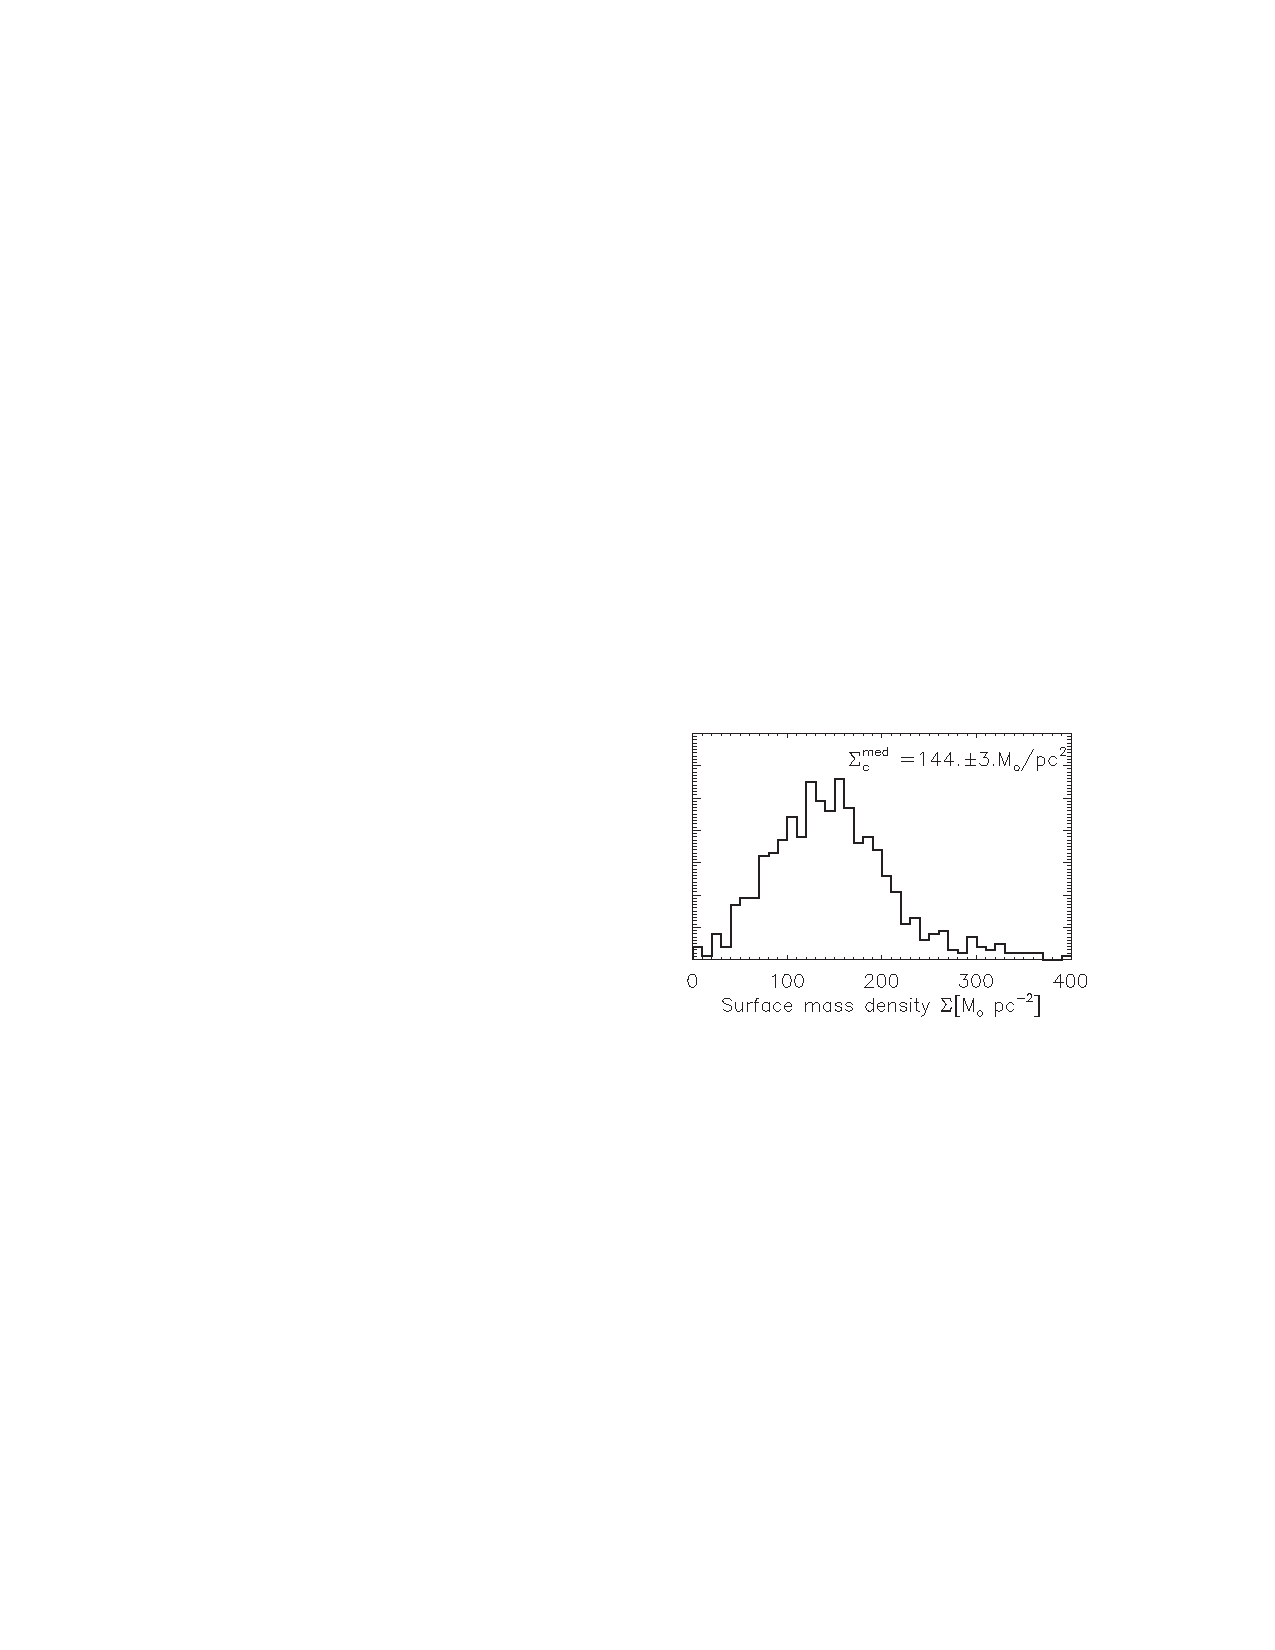
\includegraphics[width=\linewidth]{gmcsigma_roman-duval}
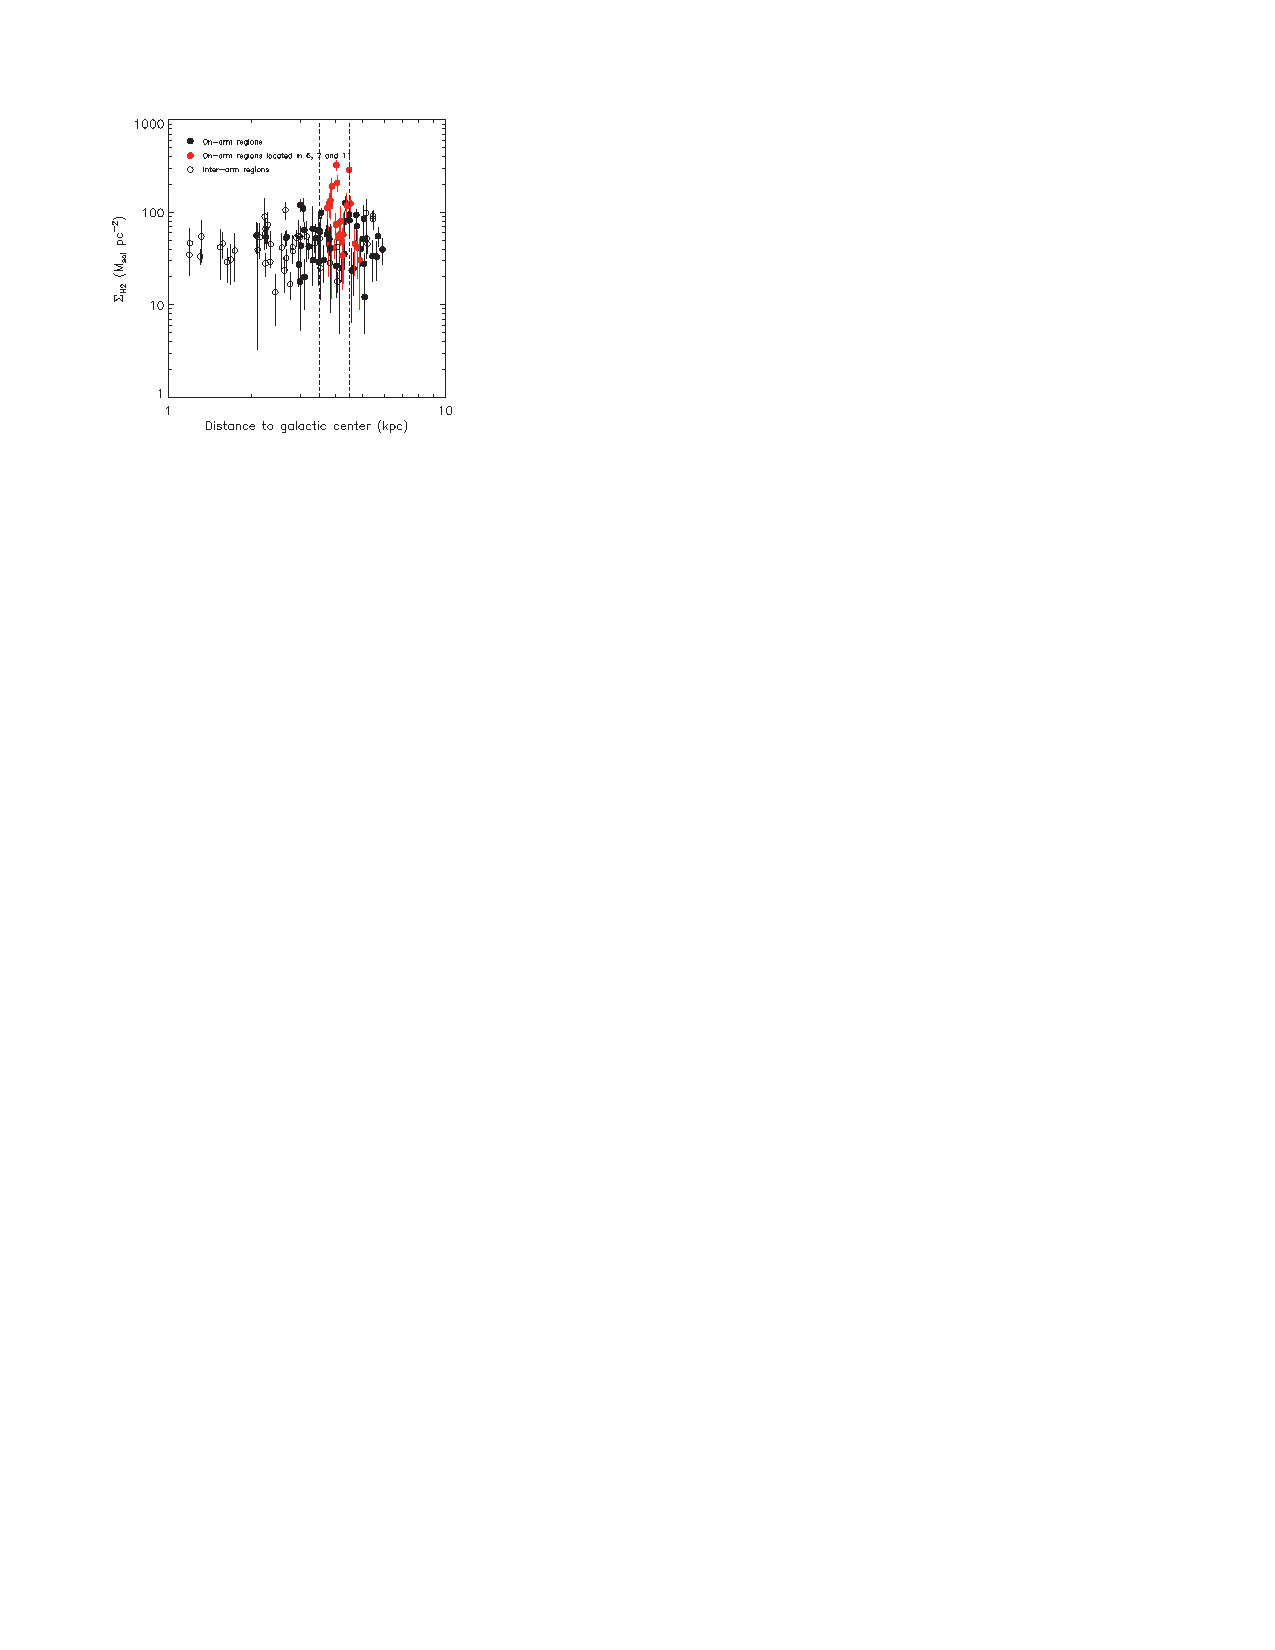
\includegraphics[width=\linewidth]{gmcsigma_rebolledo}
\caption[GMC surface densities]{
\label{fig:gmcsigma}
Two measurements of GMC surface densities. The top panel shows the distribution of surface densities for the inner Milky Way determined from $^{13}$CO measurements by \citet{roman-duval10a}. The bottom panel shows GMC surface density versus galactocentric radius in NGC 6946, measured from both $^{12}$CO and $^{13}$CO \citep{rebolledo12a}.
}
\end{marginfigure}

\begin{marginfigure}
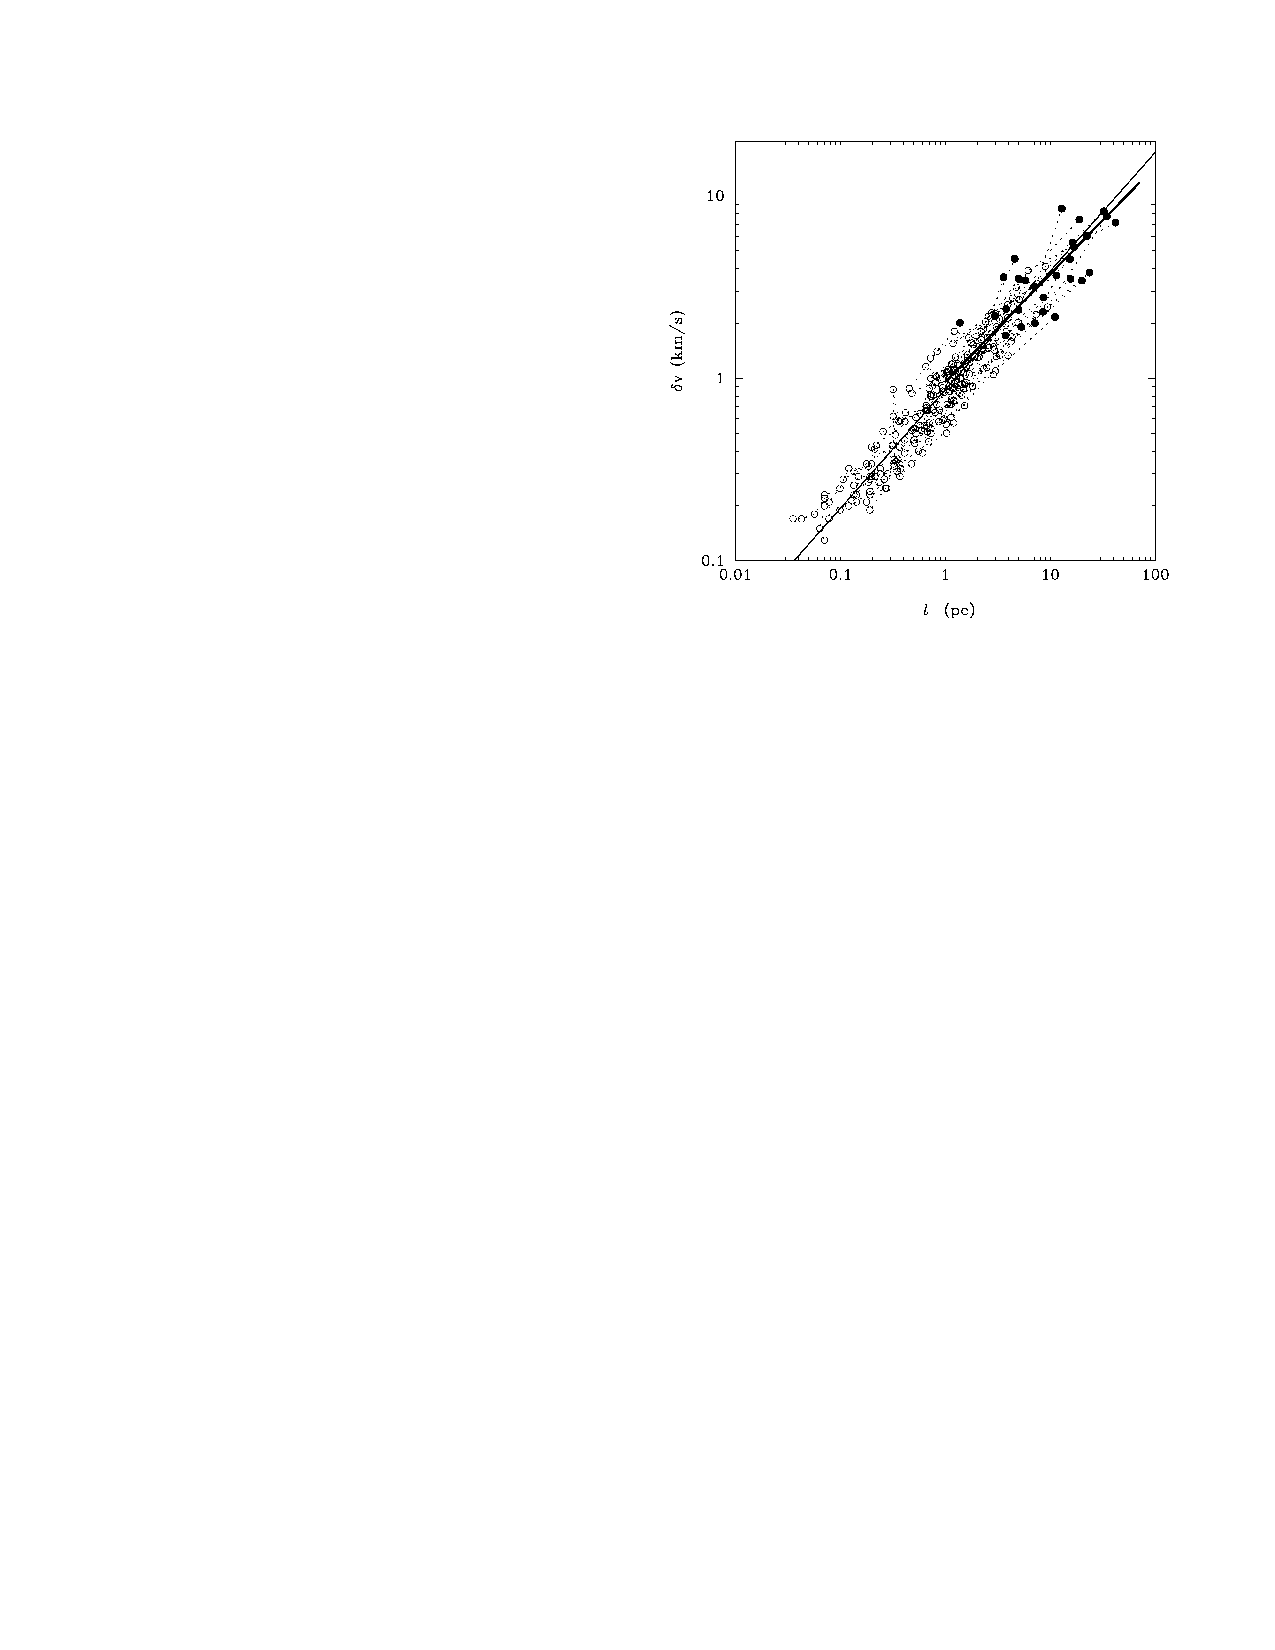
\includegraphics[width=\linewidth]{lws_heyer04}
\caption[GMC linewidth-size relation]{
\label{fig:gmclws}
Measured correlation between GMC linewidth $\delta v$ and size scale $\ell$ for Milky Way clouds \citep{heyer04a}.
}
\end{marginfigure}

One interesting thing to notice here is that the exponent of the observed linewidth-size relation within a single cloud is quite close to the scaling $\sigma\propto \ell^{0.5}$ that we expect from supersonic turbulence. However, turbulence alone does not explain why all molecular clouds follow the {\it same} linewidth-size relation, in the sense that not only is the exponent the same, but the normalization is the same. It would be fully consistent with supersonic turbulence for different GMCs to have very different levels of turbulence, so that two clouds of equal size could have very different velocity dispersions. Thus the fact that turbulence in GMCs is universal is an important observation.

Larson's final law is that GMCs have $\avir\approx 1$, i.e., they are in rough virial balance between gravity and internal turbulence. We have already noted the good agreement between the value of X that we derived from a trivial virial assumption and the value derived by $\gamma$ ray and dust observations, which suggest exactly this result. In practice, the way we compute the virial ratio is to measure a mass using an X factor calibrated by $\gamma$ rays or dust, compute a radius from the observed size of the cloud on the sky and its estimated distance, and measure the velocity dispersion from the width of the line in frequency. Using the method, \citet{solomon97a} get $\avir=1.1$ as their mean within the Galaxy, and \citet{bolatto08a} get a similar result for external galaxies. This result only appears to hold for sufficiently massive clouds. Clouds with masses below $\sim 10^4$ $\msun$ have virial ratios $\avir \gg 1$. The interpretation is that these objects are confined by external pressure rather than gravity.

It is important to realize that Larson's three laws are not independent. If we write the linewidth-size relation as $\sigma=\sigma_{\rm pc} R_{\rm pc}^{1/2}$, then
\begin{equation}
\avir = \frac{5\sigma^2 R}{G M} = \left(\frac{5}{\pi \mbox{ pc}}\right) \frac{\sigma_{\rm pc}^2}{G\Sigma} = 3.7 \left(\frac{\sigma_{\rm pc}}{1\mbox{ km s}^{-1}}\right)^2 \left(\frac{100\,\msun\mbox{ pc}^{-2}}{\Sigma}\right).
\end{equation}
This shows that the universality of the linewidth-size relation is equivalent to the universality of the molecular cloud surface density, and vice-versa. The normalization of the linewidth-size relation is equivalent to the statement that $\avir=1$, and vice-versa. This is indeed what is observed (Figure \ref{fig:gmcalpha}).

\begin{marginfigure}
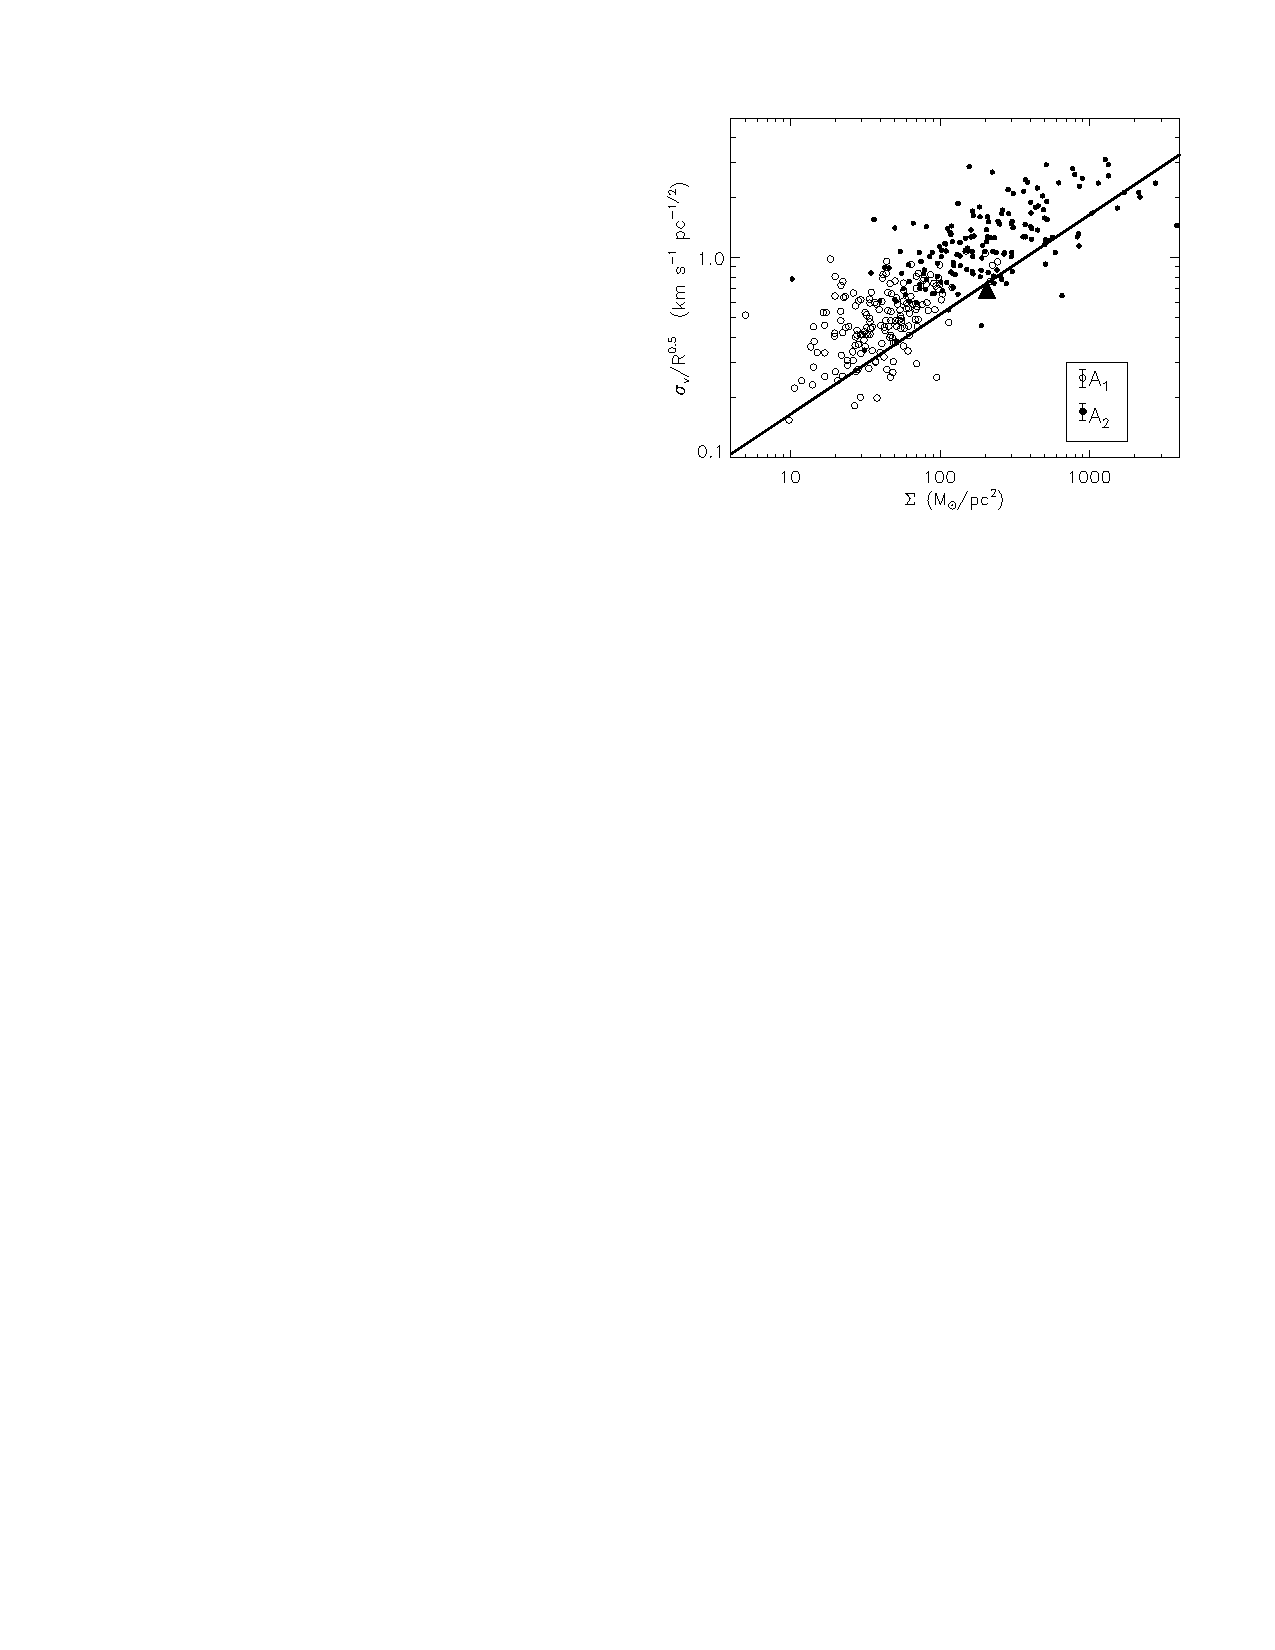
\includegraphics[width=\linewidth]{gmcalpha_heyer09}
\caption[GMC virial ratios]{
\label{fig:gmcalpha}
Correlation between GMC surface density $\Sigma$ and the combination $\sigma_v/R^{1/2}$, where $\sigma_v$ is the velocity dispersion and $R$ is the radius \citep{heyer09a}. The solid line represents the relationship that has $\alpha_{\mathrm{vir}} = 1$. Open circles indicate values derived with the lowest detectable contour, while closed ones indicate values derived using the half maximum CO isophote.
}
\end{marginfigure}

It is also instructive to compute the pressure in GMCs that these relations imply. The kinetic pressure is $P = \overline{\rho} \sigma^2 = 3\Sigma\sigma_{\rm pc}^2/(4\mbox{ pc})$ Plugging in the observed linewidth-size relation, this gives $P/k_{\rm B}\approx 3\times 10^5$ K cm$^{-3}$. This is much larger than the mean pressure in the disk of the Milky Way or similar galaxies, which is typically closer to $10^4$ K cm$^{-3}$.


\section{Molecular Cloud Timescales}

Perhaps the most difficult thing to observe about GMCs are the timescales associated with their behavior. These are always long compared to any reasonable observation time, so we must instead infer timescales indirectly. In order to help understand the physical implications of GMC timescales, it is helpful to compare these to the characteristic timescales implied by Larson's Laws.

One of these is the crossing time,
\begin{equation}
t_{\rm cr} \equiv \frac{R}{\sigma} = \frac{0.95}{\sqrt{\avir G}} \left(\frac{M}{\Sigma^3}\right)^{1/4} = 14\, \avir^{-1/2} M_6^{1/4} \Sigma_2^{-3/4}\mbox{ Myr}.
\end{equation}
This is the characteristic time that it will take a signal to cross a cloud. The other is the free-fall time,
\begin{equation}
t_{\rm ff} \equiv \sqrt{\frac{3\pi}{32 G \rho}} = \frac{\pi^{1/4}}{\sqrt{8G}}\left(\frac{M}{\Sigma^3}\right)^{1/4} = 
7.0\, M_6^{1/4} \Sigma_2^{-3/4}\mbox{ Myr}
\end{equation}
For a virialized cloud, $\avir=1$, the free-fall time is half the crossing time, and both timescales are $\sim 10$ Myr. Thus, when discussing GMCs, we will compare our timescales to 10 Myr.

\subsection{Depletion Time}

The first timescale to think about is the one defined by the rate at which GMCs form stars. We call this the depletion time -- the time required to turn all the gas into stars. Formally, $t_{\rm dep} = M_{\rm gas}/\dot{M}_*$ for a cloud, or, if we're talking about an extra-Galactic observation where we measure quantities over surface areas of a galactic disk, $t_{\rm dep} = \Sigma_{\rm gas}/\dot{\Sigma}_*$. This is sometimes also referred to gas the gas consumption timescale.

This is difficult to determine for individual GMCs, in large part because stars destroy their parent clouds after they form. This means that we do not know how much gas mass a cloud started with, just how much gas is left at the time when we observe it. If the GMC is young we might see a lot of gas and few stars, and if it is old we might see many stars and little gas, but the depletion time might be the same.

We can get around this problem by studying a galactic population of GMCs. This should contain a fair sample of GMCs in all evolutionary stages, and tell us what the value of the star formation rate is when averaged over all these clouds. \citet{zuckerman74a}, pointed out that for the Milky Way the depletion time is remarkably long. Inside the Solar circle the Milky Way contains $\sim 10^9$ $\msun$ of molecular gas, and the star formation rate in the Milky Way is $\sim 1$ $\msun$ yr$^{-1}$, so $t_{\rm dep}\approx 1$ Gyr. This is roughly 100 times the free-fall time or crossing time of $\sim 10$ Myr. \citet{krumholz05c} pointed out that this ratio is a critical observational constraint for theories of star formation, and defined the dimensionless star formation rate per free-fall time as $\epsilon_{\rm ff} = t_{\rm ff} / t_{\rm dep}$. This is the fraction of a GMC's mass that it converts into stars per free-fall time.

Since 1974 these calculations have gotten more sophisticated and have been done for a number of nearby galaxies. Probably the cleanest, largest sample of nearby galaxies comes from the recent HERACLES survey \citep{leroy13a}. Surveys of local galaxies consistently find a typical depletion time $t_{\rm dep}=2$ Gyr for the molecular gas over. A wider by lower resolution survey, COLD GASS \citep{saintonge11a, saintonge11b}, found a non-constant depletion time over a wider range of galaxies, but still relatively little variation.\footnote{It is unclear what accounts for the difference between HERACLES and COLD GASS. The samples are quite different, in that HERACLES looks at individual patches within nearby well-resolved galaxies, while COLD GASS only has one data point per galaxy, and the observations are unresolved. On the other hand, COLD GASS has a much broader range of galaxy morphologies and properties. It possible that some of the COLD GASS galaxies are in a weak starburst, while there are no starbursts present in HERACLES.} Figure \ref{fig:sfh2_krumholz14} summarizes the current observations for galaxies close enough to be resolved.


\begin{figure}
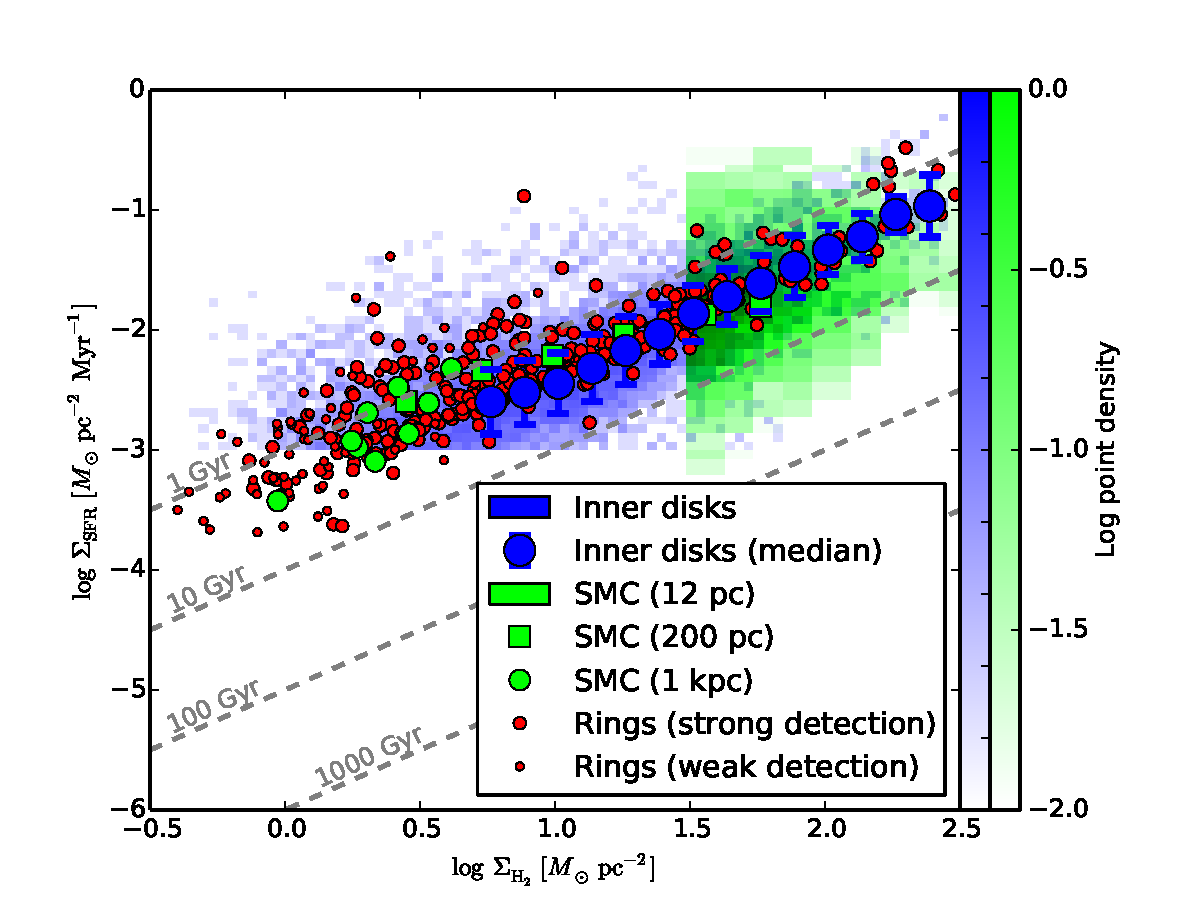
\includegraphics[width=\linewidth]{sfh2_krumholz14}
\caption[Surface densities of gas and star formation]{
\label{fig:sfh2_krumholz14}
Surface density of star formation versus surface density of gas \citep{krumholz14c}. Blue pixels show the distribution of pixels in the inner parts of nearby galaxies, resolved at $\sim 750$ pc scales \citet{leroy13a}, while green pixels show the SMC resolved at 12 pc scales \citet{bolatto11a}; other green and blue points show various averages of the pixels. Red points show azimuthal rings in outer galaxies \citet{schruba11a}, in which CO emission can be detected only by stacking all the pixels in a ring. Gray lines show lines of constant depletion time $t_{\mathrm{dep}}$.
}
\end{figure}

\citet{krumholz07e} and \citet{krumholz12a} performed this analysis for a variety of tracers of mass other than CO and for a variety of galaxies, and for individual clouds within the Milky Way, and found that $\epsilon_{\rm ff}\sim 0.01$ for essentially all of them (Figure \ref{fig:eff_krumholz14}).

\begin{figure}
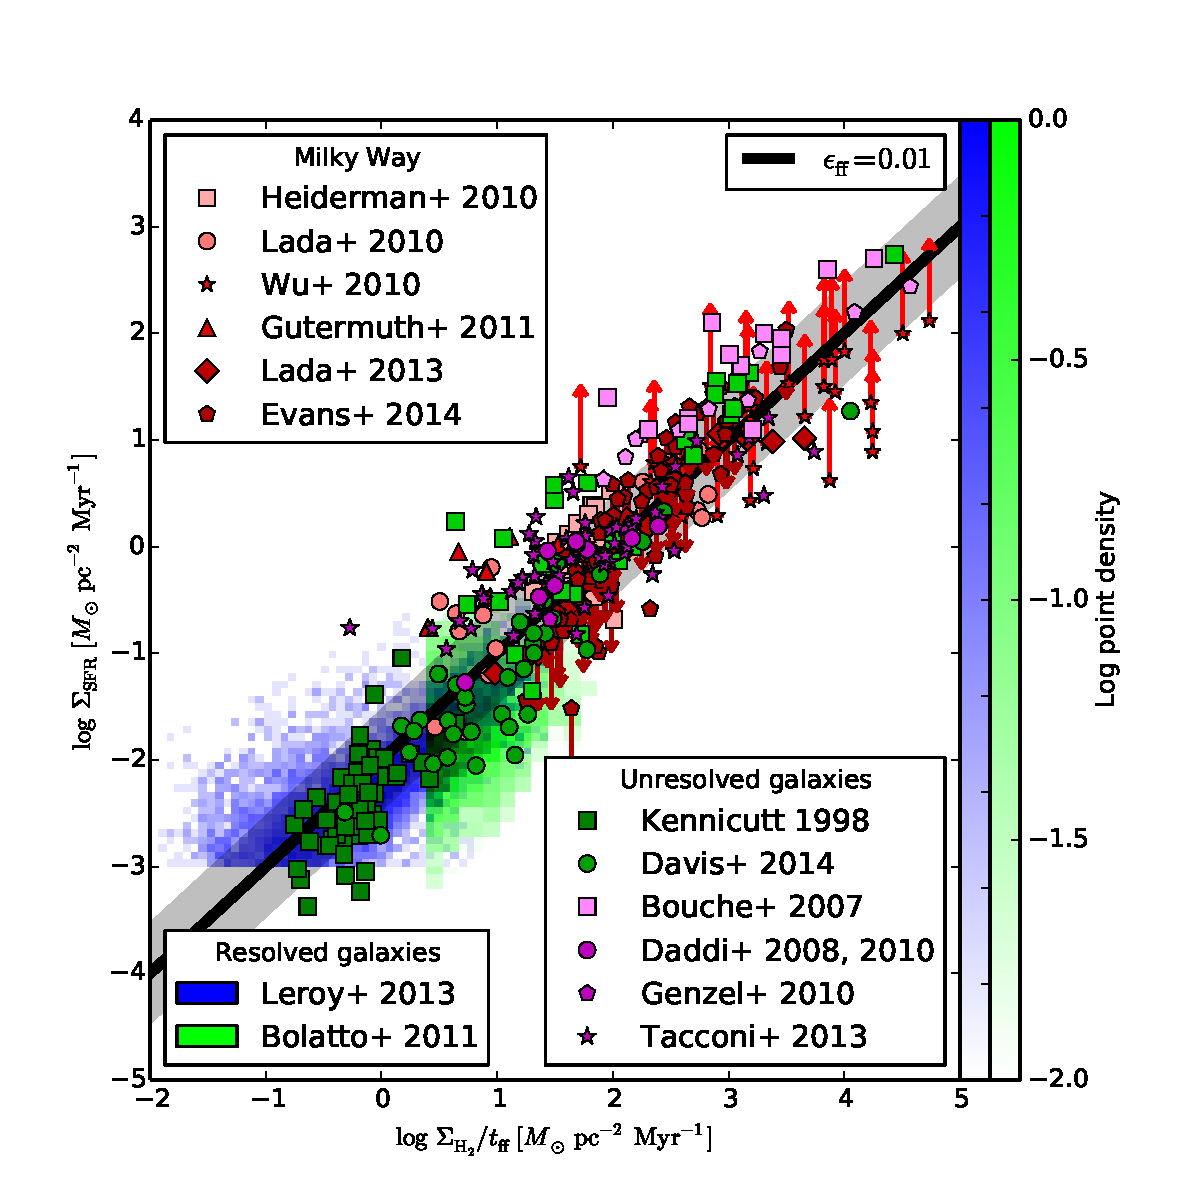
\includegraphics[width=\linewidth]{eff_krumholz14}
\caption[Surface density of star formation versus surface density of gas normalized by free-fall time]{
\label{fig:eff_krumholz14}
Surface density of star formation versus surface density of gas normalized by free-fall time \citep{krumholz14c}. Blue and green pixels are the same as in Figure \ref{fig:sfh2_krumholz14}, while points represent measurements of marginally-resolved galaxies ($\sim 1$ beam per galaxy). Points are color-coded: green indicates local galaxies, purple indicates high-$z$ galaxies, and red indicates individual Milky Way clouds. The thick black line represents $\epsilon_{\mathrm{ff}} = 0.01$, while the gray band shows a factor of 3 scatter about it.
}
\end{figure}

\subsection{Lifetime}

The second quantity of interest observationally is how long an individual GMC survives. This is a difficult problem in part because clouds are filled with structures on all scales, and authors are not always consistent regarding the scales on which a lifetime is being measured. When clouds have complex, hierarchical structures, things can depend tremendously on whether we say that a region consists of a single, sub-structured, big cloud or of many small ones. This makes it particularly difficult to compare Galactic and extra-galactic data. In extragalactic observations where resolution is limited, we tend to label things as large clouds with smaller densities and thus longer free-fall and crossing timescales. The same cloud placed within the Milky Way might be broken up and assigned much shorter timescales. The moral of this story is that, in estimating cloud lifetimes, it is important to be consistent in defining the sample and the methods used to estimate its lifetime. There are many examples in the literature of people being less than careful in this regard.

Probably the best determination of GMC lifetimes comes from extragalactic studies, where many biases and confusions can be eliminated. In the LMC, the NANTEN group catalogued the positions of all the molecular clouds \citet{fukui08a}, all the H~\textsc{ii} regions, and all the star clusters down to a reasonable completeness limit ($\sim 10^{4.5}$ $\msun$ for the GMCs). Star clusters' ages can be estimated from their colors, and thus the clusters can be broken into different age bins. They then compute the minimum projected distance between each cluster or H~\textsc{ii} region and the nearest GMC, and compare the distribution to what one would expect if the spatial distribution were random \citet[Figure \ref{fig:gmcdist_kawamura}]{kawamura09a}. There is clearly an excess of H~\textsc{ii} regions and clusters in the class SWB0, which are those with ages $\leq 10$ Myr, at small separations from GMCs. This represents a physical association between GMCs and these objects -- the clusters or H~\textsc{ii} regions are near their parent GMCs. There is no comparable excess for the older clusters. 

\begin{figure}
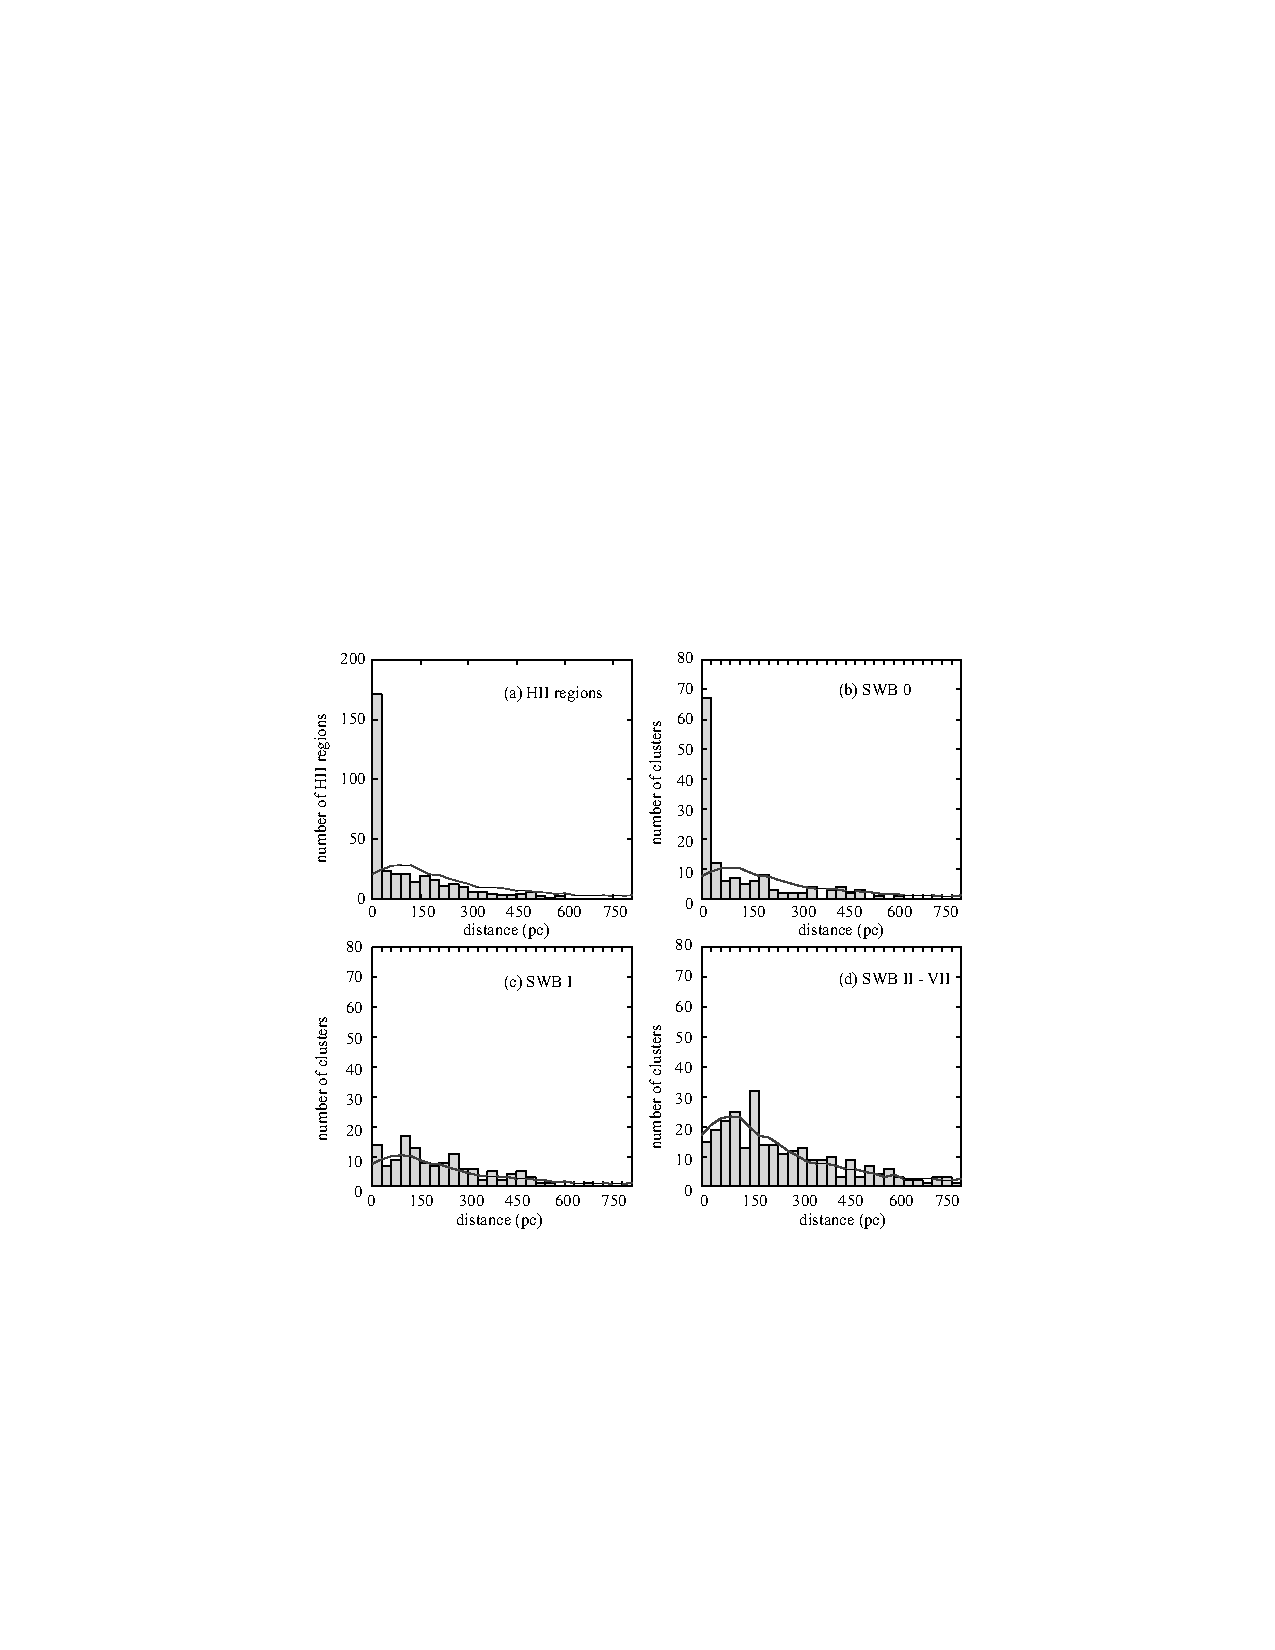
\includegraphics[width=\linewidth]{gmcdist_kawamura}
\caption[Histogram of distances to nearest GMC]{
\label{fig:gmcdist_kawamura}
Histogram of projected distances to the nearest GMC in the LMC for H~\textsc{ii} regions, star clusters $<10$ Myr old (SWB 0), star clusters $10-30$ Myr old (SWB I), and star clusters older than 30 Myr (SWB II-IV), as indicated \citep{kawamura09a}. In each panel, the lines show the frequency distribution that results from random placement of each category of object relative to the GMCs.
}
\end{figure}

This allows us to estimate the GMC lifetime as follows. First, we note that roughly 60\% of the SWB 0 clusters are in the excess spike at small separations. This implies that, on average, 60\% of their $\sim 10$ Myr lifetime must be spent near their parent GMC, i.e., the phase of a GMC's evolution when it has a visible nearby cluster is 6 Myr. To estimate the total GMC lifetime, we note that only a minority of GMCs have visible nearby clusters. \citet{kawamura09a} find 39 GMCs are associated with nearby star clusters. In contrast, 88 are associated with H~\textsc{ii} regions but not star clusters, and 44 are associated with neither. If we assume that we are seeing these clouds are random stages in their lifetimes, then the fraction associated with star clusters must represent the fraction of the total GMC lifetime for which this association lasts. Thus the lifetime of each phase is just proportional to the fraction of clouds in that phase, i.e.,
\begin{equation}
t_{\rm HII} = \frac{N_{\rm HII}}{N_{\rm cluster}} t_{\rm cluster}
\end{equation}
and similarly for $t_{\rm quiescent}$.
Plugging in the numbers of clouds, and given that $t_{\rm cluster}=6$ Myr, we obtain $t_{\rm quiescent} = 7$ Myr, $t_{\rm HII} = 14$ Myr, and $t_{\rm life} = t_{\rm starless} + t_{\rm HII} + t_{\rm cluster} = 27$ Myr. This is $\sim 2-3$ crossing times, or $4-6$ free-fall times.

Notice that for this argument to work is it {\it not} necessary that the different phases be arranged in any particular sequence. \citeauthor{kawamura09a}~suggest that there is in fact a sequence, with GMCs without clusters or HII regions forming the earliest phase, GMCs with HII regions but not clusters forming the second phase, and GMCs with both HII regions and optically visible clusters forming the third phase. However, recent theoretical work by \citet{goldbaum11a} suggests that this is not necessarily the case.

\begin{marginfigure}
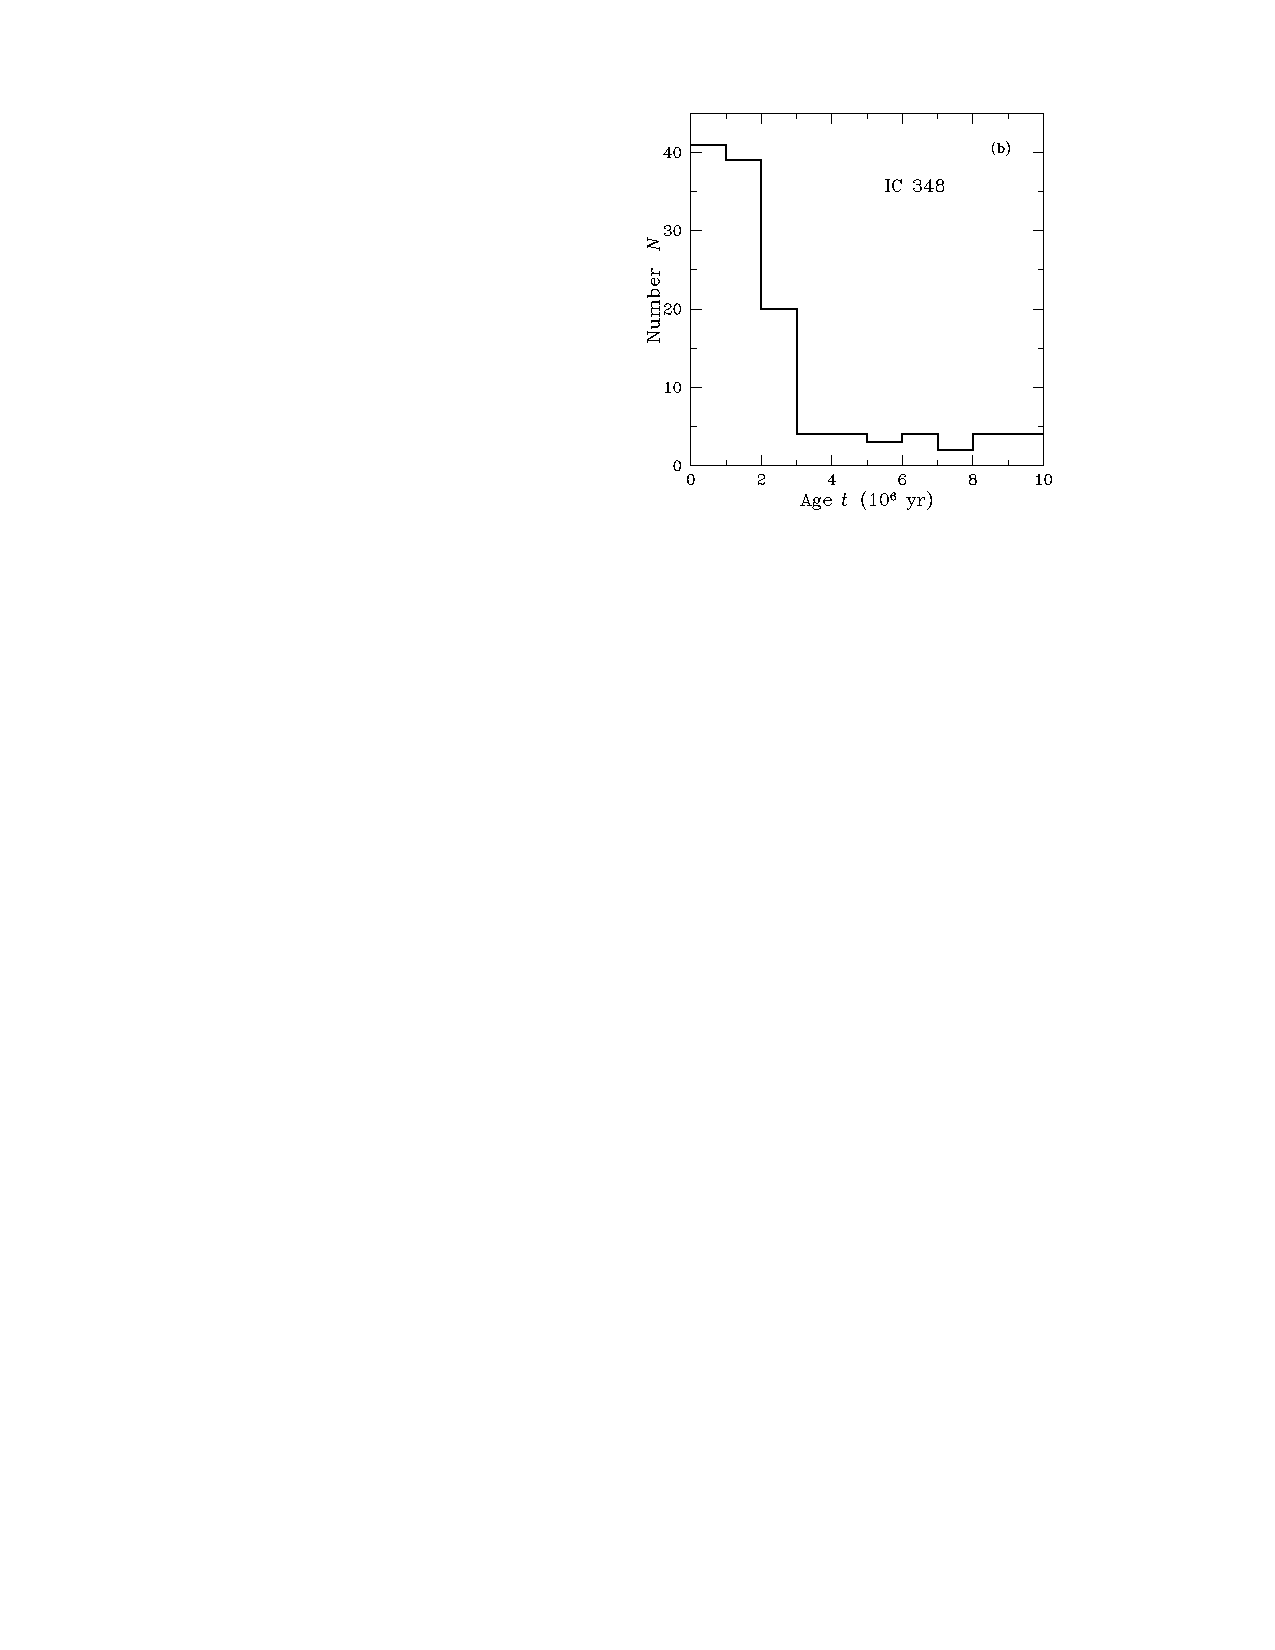
\includegraphics[width=\linewidth]{ic348_palla}
\caption[Histogram of stellar ages in IC 348]{
\label{fig:ic348_palla}
Histogram of inferred stellar ages in the cluster IC 348 \citet{palla00a}.
}
\end{marginfigure}

Within the galaxy and on smaller scales exercises like this get vastly trickier. If we look at individual star clusters, which we can age-date using pre-main sequence Hertzsprung-Russell diagrams (see Chapter \ref{ch:protostar_evol}) we find that they usually cease to be embedded in gaseous envelopes by the time the stellar population is $2-3$ Myr old (Figure \ref{fig:ic348_palla}). Interpreting this as a true cluster formation age is tricky due to numerous observational biases, e.g., variable extinction masquerading as age spread (which tends to raise the age estimate) and a bias against finding older stars because they are dimmer (which tends to reduce the age estimate). There are also uncertainties in the theoretical models themselves used to estimate the ages.

However, an individual GMC generally makes many cluster. The typical star clusters is only a few hundred $\msun$, compared to GMC masses of $10^5-10^6$ $\msun$, and we see associations made up of many clusters with age spreads of $10-15$ Myr. This suggests that the smaller pieces of a GMC (like the lumps we see in Perseus, shown in Figure \ref{fig:perseus_sun06}) clear away their gas relatively quickly, but that their larger-scale GMCs are not completely destroyed by this process.  The small regions therefore have lifetimes of a few Myr, but they also are much denser and thus have shorter crossing / free-fall times. For example, if the Orion Nebula cluster were smeared out into gas, its current stellar mass ($\sim 4000$ $\msun$) and surface density ($\Sigma \sim 0.1$ g cm$^{-2}$) suggest a crossing time of $0.7$ Myr. Given that the cluster has almost certainly lost some mass and spread out to somewhat lower surface density since it dispersed its gas, the true crossing time of the parent cloud was almost certainly shorter. This suggests an age of several crossing times for the ONC, but given the uncertainties in the true age spread of several crossing times. However, this is an extremely uncertain and controversial subject, and other authors have argued for shorter lifetimes on these smaller scales.

\subsection{Star Formation Lag Time}

A third important observable timescale is the time between GMC formation and the onset of star formation, defined as the lag time. We can estimate the lag time either statistically or geometrically. Statistically, we can do this using a technique much like what we did for the total lifetime in the LMC: compare the number of starless GMCs to the number with stars.

For the LMC, if we accept the \citet{kawamura09a} age sequence, the quiescent phase is 7 Myr. However, there may be star formation for some time before H~\textsc{ii} regions detectable at extragalactic distances begin to appear, or there may be clouds where H~\textsc{ii} regions appear and then go off, leading a cloud without a visible cluster or H~\textsc{ii} region, but still actively star-forming. This is what \citet{goldbaum11a} suggest.

In the solar neighborhood, within 1 kpc of the Sun, the ratio of clouds with star formation to clouds without is between $7:1$ and $14:1$, depending on the level of evidence on demands for star formation activity. If we take the time associated with star formation for these clouds to be $\sim 2-3$ Myr, this suggests a lag time less than a few tenths of a Myr in these high-density knots. Since this is comparable to or smaller than the crossing time, this suggests that these regions must begin forming stars while the are still in the process of forming.

Geometric arguments provide similar conclusions. The way geometric arguments work is to look at a spiral galaxy and locate the spiral shock in H~\textsc{i} or CO. Generally some tracer of star formation, e.g., H$\alpha$ emission or 24 $\mu$m IR emission, will appear at some distance behind the spiral arm. If one can measure the pattern speed of the spiral arm, then the physical distance between the spiral shock and the onset of star formation, as indicated by the tracer of choice, can be identified with a timescale. This technique is illustrated in Figure \ref{fig:sflag_tamburro08}. In effect, one wants to take this image and measure by what angle the green contours (tracing H~\textsc{i}) should be rotated so that those arms peak at the same place as the 24 $\mu$m map, and then associate a time with that.

\begin{figure}
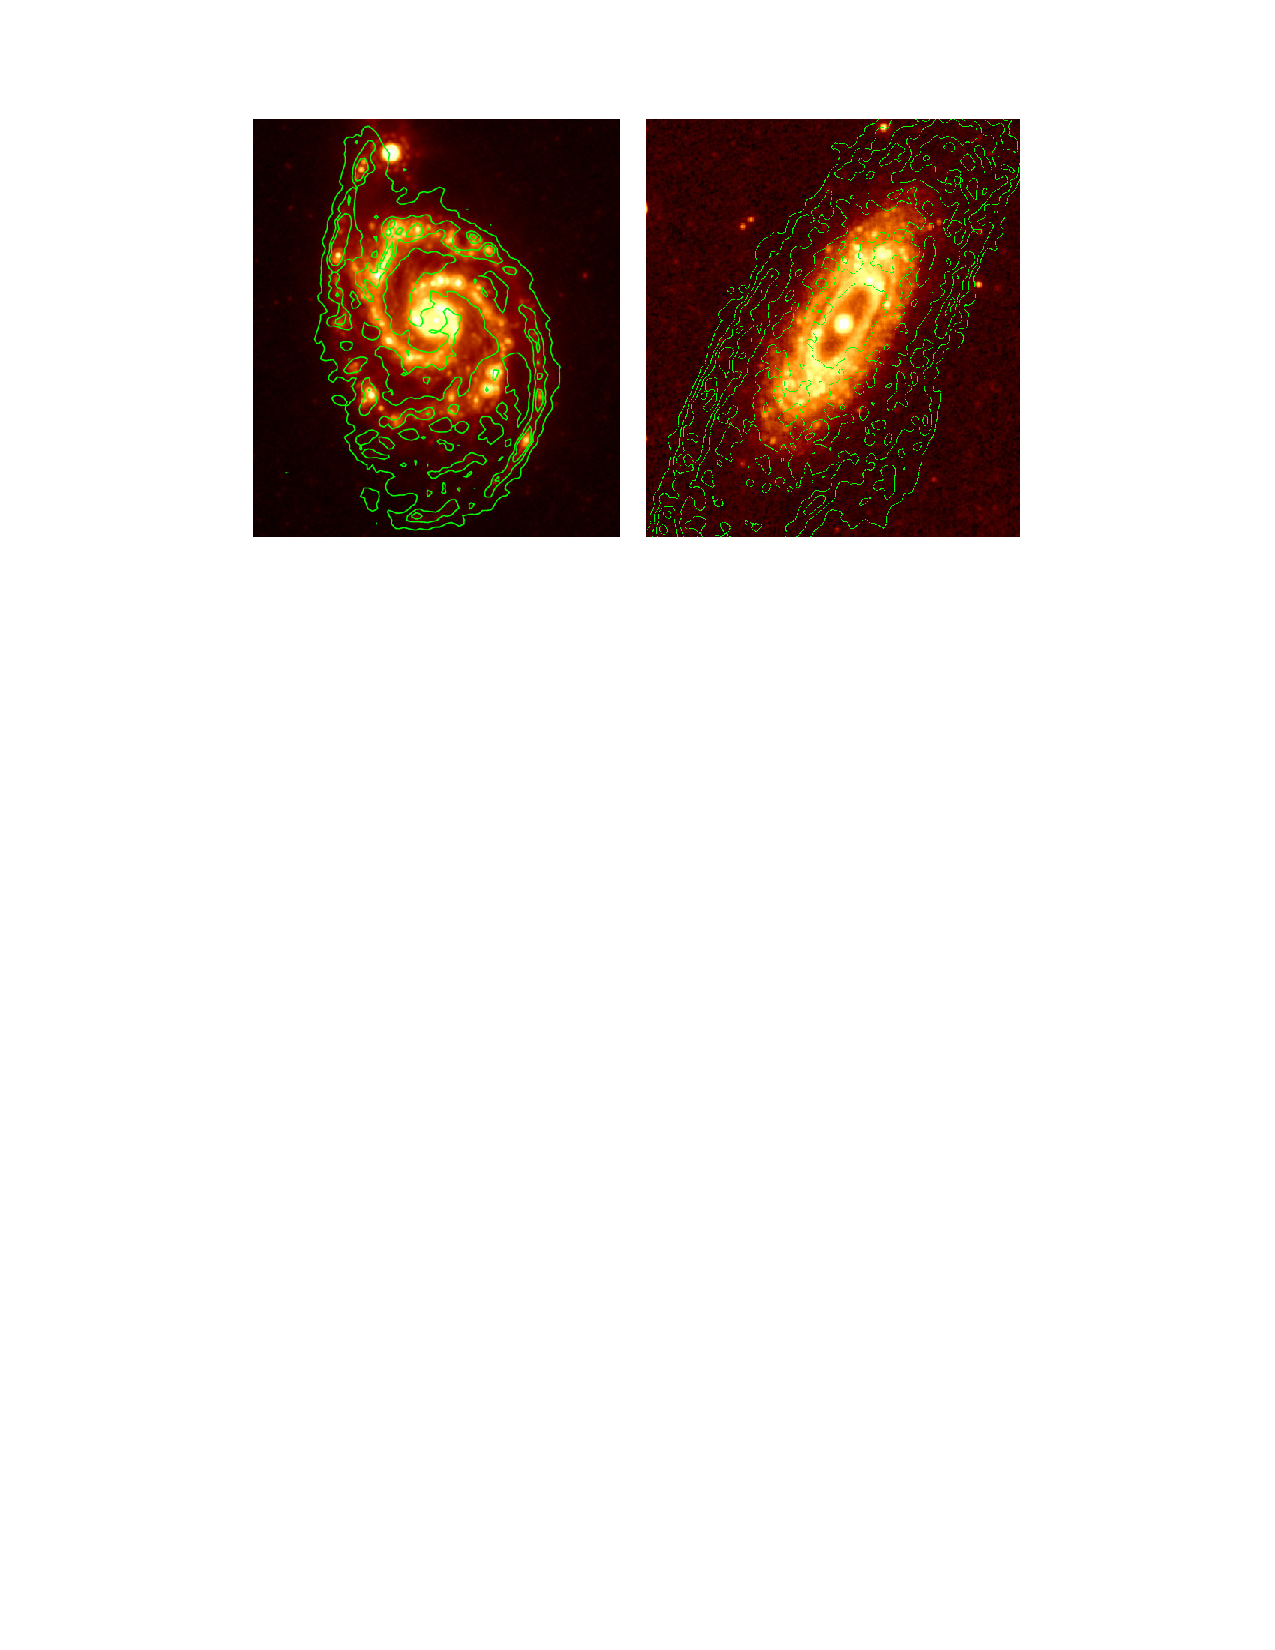
\includegraphics[width=\linewidth]{sflag_tamburro08}
\caption[H~\textsc{i} and 24 $\mu$m maps of NGC 5194 and 2841]{
\label{fig:sflag_tamburro08}
The galaxies NGC 5194 (left) and NGC 2841 (right), imaged in H~\textsc{i} from the THINGS survey with the VLA, and 24 $\mu$m from \textit{Spitzer} \citep{tamburro08a}.
}
\end{figure}

Performing this exercise with 24$\mu$m emission indicates lag timescales of $1-3$ Myr \citet{tamburro08a}. Performing it with H$\alpha$ as the tracer gives $t_{\rm lag}\sim 5$ Myr \citet{egusa04a}.The difference is probably because the H$\alpha$ better traces the bulk of the star formation, what 24 $\mu$m traces the earliest phase, when the stars are still embedded in their parent clouds. The latter is therefore probably a better estimate of the lag time. Since this is again comparable to or smaller than the molecular cloud crossing / free-fall timescale, we again conclude the GMCs must start forming stars while they are still being assembled.

